\documentclass[journal,onecolumn]{IEEEtran} % <- for draft; remove onecolumn for final

% =========================
% Packages
% =========================
\usepackage{amsmath, amssymb, amsfonts, mathtools}
\usepackage{graphicx}
\usepackage{booktabs}
\usepackage{tabularx}
\usepackage{array}
\usepackage{url}
\usepackage{hyperref}
\usepackage{xcolor}
\usepackage{pifont}
\usepackage{multirow}
\newcommand{\todo}[1]{\color{red}#1\color{black}}
\newcommand{\dani}[1]{\color{blue}#1\color{black}}

% TikZ and Libraries
\usepackage{tikz}
\usetikzlibrary{positioning, arrows.meta, shapes, shapes.geometric, fit, calc}


% =====
\usepackage{tcolorbox}
\tcbuselibrary{skins,breakable}
\usepackage[scaled=0.92]{inconsolata} % optional; remove if unavailable
\usepackage{soul}

% Soft pastel colors
\definecolor{rolebg}{RGB}{226,238,255}
\definecolor{contextbg}{RGB}{226,242,226}
\definecolor{taskbg}{RGB}{255,239,210}
\definecolor{outputbg}{RGB}{240,228,246}
\definecolor{headbg}{RGB}{248,248,248}

% Main figure box
\newtcolorbox{promptfigure}[2][]{%
  enhanced,
  sharp corners,
  colback=white,
  colframe=black,
  colbacktitle=headbg,
  coltitle=black,
  boxrule=0.5pt,
  title={#2},
  fonttitle=\bfseries,
  left=1mm,right=1mm,top=0.8mm,bottom=0.8mm,
  boxsep=0.5mm,
  before skip=4pt,
  after skip=4pt,
  colbacklower=gray!2,
  segmentation style={solid, black, line width=0.35pt},
  #1
}

% Tiny legend chip
\newtcbox{\legendchip}[1][]{%
  on line,
  boxrule=0.35pt,
  colframe=black,
  colback=gray!15,
  arc=1pt,
  left=2pt,right=2pt,top=0.5pt,bottom=0.5pt,
  boxsep=0pt,
  fontupper=\scriptsize\bfseries,
  #1
}


% Output lines
\newcommand{\outputline}[1]{{\ttfamily #1}\par}

% =======
\definecolor{exonebg}{RGB}{232,241,255}
\definecolor{extwobg}{RGB}{232,247,236}
\definecolor{targetbg}{RGB}{255,243,220}
\definecolor{reasonbg}{RGB}{255,239,210}
\definecolor{retrievedbg}{RGB}{236,232,248}
\definecolor{querybg}{RGB}{233,244,255}



\newcommand{\rolehl}[1]{{\sethlcolor{rolebg}\hl{#1}}}
\newcommand{\contexthl}[1]{{\sethlcolor{contextbg}\hl{#1}}}
\newcommand{\taskhl}[1]{{\sethlcolor{taskbg}\hl{#1}}}
\newcommand{\outputhl}[1]{{\sethlcolor{outputbg}\hl{#1}}}
\newcommand{\exonehl}[1]{{\sethlcolor{exonebg}\hl{#1}}}
\newcommand{\extwohl}[1]{{\sethlcolor{extwobg}\hl{#1}}}
\newcommand{\targethl}[1]{{\sethlcolor{targetbg}\hl{#1}}}
\newcommand{\reasonhl}[1]{{\sethlcolor{reasonbg}\hl{#1}}}
\newcommand{\retrievedhl}[1]{{\sethlcolor{retrievedbg}\hl{#1}}}
\newcommand{\queryhl}[1]{{\sethlcolor{querybg}\hl{#1}}}

\newcommand{\goodmark}{\textcolor{green!50!black}{\ding{51}}}
\newcommand{\badmark}{\textcolor{red!70!black}{\ding{55}}}
% ++++
\newcommand{\neutralprompt}[1]{{\ttfamily #1\par\vspace{0.2mm}}}


\usepackage{ragged2e}
\newcolumntype{Y}{>{\RaggedRight\arraybackslash}X}
\newcolumntype{P}[1]{>{\RaggedRight\arraybackslash}p{#1}}

% =========================
% Title
% =========================
\title{LLMs and Agentic Systems for Smart Grids: Applications and Architectures}

\author{
Daniela~Rojas, Yuanyuan~Shi
% other team case study contributors
}

\begin{document}
\maketitle

% =========================
% Abstract
% =========================
\begin{abstract}
Agentic AI systems are starting to support complex engineering workflows. In smart grids, large language models (LLMs) can help specify tasks, call tools, explain results, and draft reports. However, grid workflows are solver-centered: numerical correctness and constraint satisfaction must remain grounded in trusted optimization and simulation tools.
This paper presents a practitioner oriented framework for designing large language model (LLM) and agentic AI systems for smart grid applications. We describe three system layers 1) prompting-only systems (including structured prompting, few-shot prompting, chain-of-thought, and retrieval-augmented generation), 2)single-agent systems (including ReAct, Plan-and-Act, hierarchical, self-reflection, and multi-agent architectures), and 3) fine-tuning and alignment methods.  Four case studies ground the framework in concrete implementations: an LLM-based wind power forecasting system, a solar investment agent, an EV charging scheduling agent (AgenticEV), and a multi-turn power flow analysis agent (PFAgent). Across these case studies, solver-grounded agents match or closely approach the performance of direct numerical solvers while exposing natural-language interfaces, whereas standalone LLMs fail on constrained numerical tasks despite fluent text generation. We also propose a solver-grounded evaluation protocol that emphasizes feasibility, faithfulness to tool outputs, safe failure behavior, and tool-call cost.
\end{abstract}

\begin{IEEEkeywords}
Agentic AI, large language models, smart grids, power systems, tool use, verification, retrieval-augmented generation, fine-tuning, EV scheduling, power flow analysis.
\end{IEEEkeywords}

% ============================================================
\section{Introduction}
\label{sec:intro}
Power system operation is solver-centered: engineers and operators define a model, run trusted optimization or simulation tools, check constraints, and then decide actions. As grid complexity grows (driven by distributed energy resources (DERs), renewable variability, demand flexibility, and increasing data volumes) this workflow demands faster iteration, more automated debugging, and clearer reporting to operators and stakeholders. Large language models (LLMs) offer a new interface layer for these workflows, can parse natural-language requests, generate and explain code, retrieve domain knowledge, and synthesize reports from structured numerical outputs. However, LLM outputs alone do not enforce physical laws or operational constraints. A fluent language model can describe a dispatch schedule or a power flow result in detail while still reporting a physically infeasible or numerically incorrect answer. The challenge for smart grid AI systems is therefore not capability but correctness: how to combine the language interface strengths of LLMs with the numerical reliability of established solvers and simulators.

This paper addresses that challenge by focusing on \emph{agentic AI systems} for smart grids: systems that can plan steps, call trusted tools, store intermediate results, verify constraints, and iterate until a valid result is obtained. In these systems, large language models (LLMs) are a key component, but not the source of numerical truth. We formalize this view with a solver-grounded design rule: a numerical result is reported only if it comes from a trusted tool and passes verification.


Recent work connects LLMs to external tools for grounded reasoning~\cite{yao2023react,schick2023toolformer}, studies agent loops with feedback and self-correction~\cite{shinn2023reflexion}, and proposes multi-agent coordination protocols~\cite{wu2023autogen}. In the power systems domain, capability studies have benchmarked LLMs on OPF, EV scheduling, forecasting, and retrieval tasks~\cite{huang2024foundation,majumder2024electric}, and system-level papers have introduced working agentic architectures for specific grid problems~\cite{jin2025gridmind,zhang2025gridagent,chen2025xgridagent,zhang2025poweragent,jia2025feedback}. This paper complements those contributions by providing the design guidance and evaluation protocol that practitioners need to build, and deploy these systems reliably.

%This paper provides a structured view of LLM-based and agentic approaches for smart grids. We propose a layered taxonomy and a solver-grounded system abstraction where numerical results are reported only if they come from trusted tools and pass verification checks. We map representative grid applications to these layers, present reference architectures, and outline evaluation metrics focused on feasibility, faithfulness to tool outputs, safe failure behavior, and tool-call cost.

The main contributions of this paper are:

\begin{itemize}
  \item A solver-grounded design rule and a layered taxonomy spanning prompting and LLM Agents.
  \item A reference framework that maps representative smart grid problems to system layers, architectures, and design patterns.
  \item Five concrete case studies, wind power forecasting, solar investment advising, EV scheduling, and power flow analysis, that empirically validate the solver-grounded principle.
  \item A repeatable evaluation protocol for feasibility, faithfulness to tool outputs, safe failure behavior, and tool-call cost.
\end{itemize}

The remainder of the paper is organized as follows. Section~\ref{sec:workflow} formalizes the solver-grounded workflow and reviews related work. Section~\ref{sec:prompting} covers prompting systems with worked examples. Section~\ref{sec:agents} covers agentic architectures, tool use, memory, and frameworks. Section~\ref{sec:casestudies} presents the four case studies. Section~\ref{sec:SFT_RL} covers fine-tuning, alignment, and the evaluation protocol. Section~\ref{sec:conclusion} concludes with open problems and future directions.

% ============================================================
\section{Solver-Centered Workflows and the Role of Agentic AI}
\label{sec:workflow}
% ============================================================
Power system analysis workflows are organized around trusted numerical tools: a solver or simulator computes the operating point, a checker verifies the result, and a human or automated controller acts on it. This section formalizes that workflow, identifies where LLMs and agents add value without displacing the solver, and positions this paper relative to recent related work.

% ============================================================

\begin{figure}[ht]
\centering
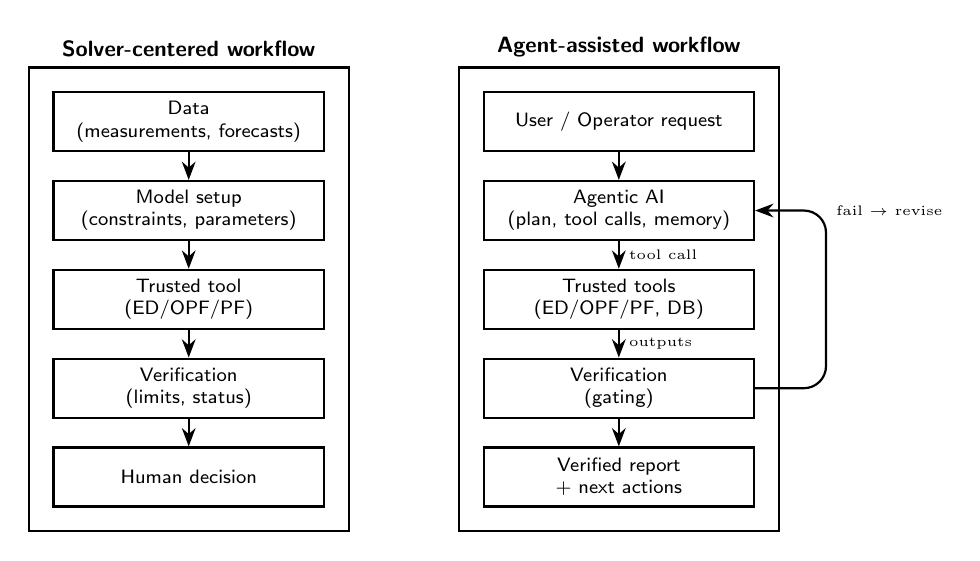
\begin{tikzpicture}[
    node distance=0.35cm and 0.7cm,
    block/.style={
        rectangle, draw=black, thick, fill=white,
        text width=3.2cm, align=center,
        minimum height=0.75cm, font=\sffamily\scriptsize
    },
    arrow/.style={-{Stealth[scale=1.0]}, thick}
]

% Left: canonical solver workflow
\node[block] (dataL) {Data \\ (measurements, forecasts)};
\node[block, below=of dataL] (modelL) {Model setup \\ (constraints, parameters)};
\node[block, below=of modelL] (solverL) {Trusted tool \\ (ED/OPF/PF)};
\node[block, below=of solverL] (verifyL) {Verification \\ (limits, status)};
\node[block, below=of verifyL] (humanL) {Human decision};

\draw[arrow] (dataL) -- (modelL);
\draw[arrow] (modelL) -- (solverL);
\draw[arrow] (solverL) -- (verifyL);
\draw[arrow] (verifyL) -- (humanL);

\node[draw, thick, inner sep=0.3cm, fit=(dataL)(humanL),
label={[font=\sffamily\bfseries\footnotesize]north:Solver-centered workflow}] (boxL) {};

% Right: agent-assisted workflow
\node[block, right=2.0cm of dataL] (userR) {User / Operator request};
\node[block, below=of userR] (agentR) {Agentic AI \\ (plan, tool calls, memory)};
\node[block, below=of agentR] (toolsR) {Trusted tools \\ (ED/OPF/PF, DB)};
\node[block, below=of toolsR] (verifyR) {Verification \\ (gating)};
\node[block, below=of verifyR] (reportR) {Verified report \\ + next actions};

\draw[arrow] (userR) -- (agentR);
\draw[arrow] (agentR) -- node[right, font=\tiny] {tool call} (toolsR);
\draw[arrow] (toolsR) -- node[right, font=\tiny] {outputs} (verifyR);
\draw[arrow] (verifyR) -- (reportR);

% feedback loop
\draw[arrow, rounded corners=8pt] (verifyR.east) -- ++(0.9,0) |- node[right, font=\tiny] {fail $\rightarrow$ revise} (agentR.east);

\node[draw, thick, inner sep=0.3cm, fit=(userR)(reportR),
label={[font=\sffamily\bfseries\footnotesize]north:Agent-assisted workflow}] (boxR) {};

\end{tikzpicture}
\caption{Left: a canonical solver-centered workflow in which data flows through model setup, a trusted solver, and a verification step before a human decision. Right: an agent-assisted workflow in which the LLM orchestrates the same steps through tool calls. The feedback arrow (fail $\rightarrow$ revise) is the key addition: the agent can retry when verification fails, but reported numbers are always gated by the verification step.}
\label{fig:workflow_two_panel}
\end{figure}

\subsection{Solver-grounded verification and reporting}
The central design rule of this paper is: \textbf{report a numerical result only if it is tool-derived and passes verification.} Let $T_k$ be a trusted tool (solver or simulator) and let $z = T_k(x)$  denote its output given input $x$. Let $\mathcal{V}$ be a set of  checks (solver status, constraint violations, unit sanity). The  verification result is $v = \mathcal{V}(z) \in \{\text{pass},\text{fail}\} \times \mathbb{R}^m$. A system is solver-grounded if any reported numerical result is based  on a $z$ with $v = \text{pass}$. Fig.~\ref{fig:workflow_two_panel} shows how an agentic AI layer wraps the canonical solver-centered workflow: the agent orchestrates tool calls and may iterate on failure, but the verification gate is never bypassed before reporting. This rule has a direct corollary for failure handling: when $v = \text{fail}$, the system should state the failure explicitly (with the violation or status message) rather than fabricate or extrapolate a number. Safe failure behavior,  refusing to report rather than hallucinating, is therefore a first-class design requirement alongside accuracy.


\subsection{Where LLMs and agents help most}
%\dani
{In smart grids, LLMs are useful because many tasks mix numbers, rules, and text, such as event logs, operating manuals, and operator reports. Recent domain studies already show that LLMs can support a broad range of power-system tasks. Large foundation model studies have evaluated tasks such as optimal power flow, electric-vehicle scheduling, technical-report retrieval, and situation awareness \cite{huang2024foundation}. Broader analyses of the electric energy sector also discuss power-flow and OPF analysis, forecasting, code generation, multimodal diagnostics, data analysis, and retrieval-augmented question answering over technical knowledge bases \cite{majumder2024electric}. Related work further shows that LLMs can generate simple OpenDSS distribution feeders for educational load-flow studies, illustrating their usefulness as interface and modeling assistants even in power-engineering settings \cite{bonadia2023potential}. Taken together, these results suggest that prompting systems are most useful for knowledge-intensive reasoning, engineering question answering, report support, and limited numerical or coding assistance, but they should not be treated as standalone sources of physically valid grid decisions \cite{huang2024foundation,majumder2024electric}.}

Common workflow bottlenecks include model setup, infeasibility debugging, scenario iteration, and report writing. Agentic AI can reduce time at each of these stages, but it should not replace the solver. Table~\ref{tab:bottlenecks} maps the principal bottlenecks to solver-grounded LLM support patterns and the corresponding sections of this paper.



\begin{table}[ht]
\centering
\caption{Workflow bottlenecks and solver-grounded LLM/agent support.}
\label{tab:bottlenecks}
\begin{tabularx}{\linewidth}{l l X p{2.0cm}}
\toprule
\textbf{Stage} & \textbf{Bottleneck} & \textbf{Solver-grounded support} & \textbf{Covered in} \\
\midrule
Data preparation & Missing values, unit mismatches 
  & Validation checks, unit normalization, schema parsing 
  & Section \ref{sec:agents} \\
Model setup & Wrong limits, inconsistent assumptions 
  & Templates, retrieval of assumptions (RAG), sanity checks 
  & Section \ref{sec:prompting} \\
Tool run & Infeasible/non-converged cases 
  & Tool orchestration, bounded retries, log parsing 
  & Section \ref{sec:agents} \\
Verification & Violations missed or misread 
  & Automated checks + max-violation summary 
  & Section \ref{sec:agents} \\
Iteration & Many what-if runs 
  & Planning, batching, caching, structured comparison 
  & Section \ref{sec:agents} \\
Reporting & Hard to explain outputs 
  & Faithful summaries tied to verified tool outputs 
  & Section \ref{sec:prompting}, \ref{sec:agents} \\
\bottomrule
\end{tabularx}
\end{table}

\subsection{Related approaches}
\label{sec:related}
%Capability studies of LLMs in the electric energy sector established the empirical baseline this work builds on. Majumder et al.\ evaluate LLM performance on power-flow analysis, OPF, forecasting, code generation, and retrieval-augmented question answering, and identify the persistent gap between fluent text generation and physically grounded computation~\cite{majumder2024electric}. Huang et al.\ evaluate foundation models on optimal power flow, EV scheduling, technical-report retrieval, and situational awareness~\cite{huang2024foundation}. Amjad et al.\ provide a taxonomy of LLM applications across the electrical power and energy sector, covering fault diagnosis, demand response, and market operations~\cite{amjad2025review}. Khalid et al.\ introduce the Agentic Digital Twin concept and survey fine-tuning and adaptation approaches for energy-sector foundation models~\cite{agentic_dt_2025}. These studies document what LLMs can do in the energy domain, but none provides design guidance for practitioners building these systems, a formal verification rule, or an evaluation protocol grounded in solver outputs.

\paragraph{Capability studies}
Majumder et al.\ evaluate LLM performance on power-flow analysis, OPF, forecasting, code generation, and retrieval-augmented question answering, and identify the persistent gap between fluent text generation and physically grounded computation~\cite{majumder2024electric}. Huang et al.\ evaluate foundation models on optimal power flow, EV scheduling, technical-report retrieval, and situational awareness~\cite{huang2024foundation}. Amjad et al.\ provide a taxonomy of LLM applications across the electrical power and energy sector, covering fault diagnosis, demand response, and market operations~\cite{amjad2025review}. Khalid et al.\ introduce the Agentic Digital Twin concept and survey fine-tuning and adaptation approaches for energy-sector foundation models~\cite{agentic_dt_2025}.

%At the system level, recent papers present working agentic architectures for specific power-system tasks. GridMind integrates LLMs with deterministic solvers through a multi-agent architecture for AC OPF and N-1 contingency analysis~\cite{jin2025gridmind}. Grid-Agent introduces an autonomous violation-detection and remediation framework combining a planning agent with a sandboxed validation agent~\cite{zhang2025gridagent}. X-GridAgent implements a three-layer hierarchical architecture for power system analysis through natural-language queries~\cite{chen2025xgridagent}. PowerAgent proposes a roadmap organized around foundation models, Model Context Protocol interfaces, and agentic workflows~\cite{zhang2025poweragent}. Jia et al.\ propose a feedback-driven multi-agent framework using error-signal feedback to improve solver accuracy~\cite{jia2025feedback}.
%These system papers make important empirical contributions on specific tasks, but they do not explain how practitioners should choose between agent architectures for a given grid workflow, compare prompting strategies with worked examples, or specify how to evaluate faithfulness and safe failure across solver-centered pipelines.

\paragraph{System-level architectures}
GridMind integrates LLMs with deterministic solvers through a multi-agent architecture for AC OPF and N-1 contingency analysis~\cite{jin2025gridmind}. Grid-Agent introduces an autonomous violation-detection and remediation framework combining a planning agent with a sandboxed validation agent~\cite{zhang2025gridagent}. X-GridAgent implements a three-layer hierarchical architecture for power system analysis through natural-language queries~\cite{chen2025xgridagent}. PowerAgent proposes a roadmap organized around foundation models, Model Context Protocol interfaces, and agentic workflows~\cite{zhang2025poweragent}. Jia et al.\ propose a feedback-driven multi-agent framework using error-signal feedback to improve solver accuracy~\cite{jia2025feedback}.

\paragraph{Gap addressed by this paper}
The capability studies document what LLMs can do, but provide no design guidance for building systems or evaluation grounded in solver outputs. The system papers make important empirical contributions on specific tasks, but do not compare prompting strategies with worked examples, explain how to choose between agent architectures, or specify how to evaluate faithfulness and safe failure across solver-centered pipelines. This paper addresses that gap by providing a \textit{practitioner-oriented framework}: a structured treatment of the full design space from prompting to multi-agent coordination, with worked power-system examples at each layer, four case studies, and a repeatable evaluation protocol grounded in the solver-verification rule of Section~\ref{sec:workflow}.

%This paper addresses that gap directly. Rather than surveying what exists, it provides a \textit{practitioner-oriented framework}: a structured treatment of the full design space from prompting to multi-agent coordination, with worked power-system examples at each layer and a repeatable evaluation protocol grounded in the solver-verification rule introduced in Section~\ref{sec:workflow}.

% ============================================================
%\newpage
\section{Prompting Systems for Smart Grids}
\label{sec:prompting}
% ============================================================

This section covers systems where the LLM output is produced by prompting, including improvements through few-shot prompting, chain-of-thought, and retrieval-augmented generation. These methods are useful for modeling tasks and for language interface support, but they do not enforce grid feasibility by themselves.

\subsection{LLM basics}
Large language models are probabilistic sequence models trained to predict the next token from the previous tokens \cite{brown2020language,vaswani2017attention}. Formally, for a token sequence $x_{1:T}$, the model defines
\begin{equation}
p(x_{1:T}) = \prod_{t=1}^{T} p(x_t \mid x_{<t}).
\end{equation}
During pretraining, the model parameters $\theta$ are optimized on a large text corpus by maximizing the likelihood of the training sequences, or equivalently by minimizing the negative log-likelihood:
\begin{equation}
\label{loss_predict}
\mathcal{L}_{\text{pre}}(\theta)
= - \sum_{x \in \mathcal{D}} \sum_{t=1}^{T}
\log p_{\theta}(x_t \mid x_{<t}),
\end{equation}

% WRITE THE OBJECTION FUCNTION IN THE PRE TRAINNING. 

% \todo{have a few sentences to briefly describe the overall training pipeline of the commons LLM models in Table II: self-supervised pre-training (which your next token prediction loss (3)); the SFT; then RL finetuning/alignment... Then mention we will talk about the SFT and alignment in Section V} 
where $\mathcal{D}$ is the pretraining dataset. {LLMs in Table \ref{tab:llm_families} follow a common training pipeline. The first stage is self-supervised pretraining using the next-token prediction loss in (\ref{loss_predict}). The pretrained model is then adapted by supervised fine-tuning (SFT) on instruction-response data so that it can generate responses with better quality.} {A final alignment stage is often applied, for example through reinforcement learning from human feedback (RLHF), to improve instruction following and safety \cite{ouyang2022training}. We discuss SFT and alignment further in Section \ref{sec:SFT_RL}.}
%After pretraining, the model can be instruction tuned so that it follows tasks written in natural language. 

LLMs are useful for many tasks, such as summarization, question answering, and explanation. However, the LLM model alone does not guarantee its output satisfies physical laws, solution feasibility or optimality. As a result, a standalone LLM may produce fluent text and still give a numerically wrong or infeasible grid dispatch/control actions. Therefore, prompting-only systems are better viewed as support tools for smart grid tasks in natural language, such as reasoning, explanation, and interface tasks, not as final decision makers. 

% In smart grids, this flexibility is useful because many tasks mix numbers, rules, and text, such as event logs, operating manuals, and operator reports. \todo{This is a good place to cite some papers, such as ``Large foundation models for power systems'', ``Exploring the capabilities and limitations of large language models in the electric energy sector'', and there are several more. Review the power system tasks they have exploited } \dani{Done}


\subsection{Representative frontier LLM families}
\begin{table*}[tb]
\centering
\footnotesize
\caption{{Representative frontier LLM families for prompting and agentic systems.
For proprietary models, parameter counts are listed as not publicly disclosed because official provider documentation does not report them.}}
\label{tab:llm_families}
\renewcommand{\arraystretch}{1.15}
\setlength{\tabcolsep}{4pt}
\begin{tabularx}{\textwidth}{p{1.4cm} p{2cm} p{1.5cm} p{1.5cm} p{2cm} p{2.2cm} X}
\toprule
\textbf{Access type} & \textbf{Model family} & \textbf{Provider} & \textbf{Parameters} & \textbf{Context window} & \textbf{Modalities} & \textbf{Capabilities} \\
\midrule

\multirow{4}{*}{\parbox{1.5cm}{\centering Proprietary}}
& GPT-5.4 & OpenAI & --- & 1.0M tokens & Text, image & Function calling, hosted tools, and strong support for long-running agentic workflows. \\
& Claude Sonnet 4.6 & Anthropic & --- & 1M tokens & Text, image & Long-context reasoning, agent planning, computer use, and programmatic tool calling. \\
& Gemini 3.1 Pro Preview & Google & --- & 1,048,576 tokens & Text, image, video, audio & Function calling, code execution, search grounding, and multimodal reasoning. \\
& Grok 4.20 & xAI & --- & 2M tokens & Text, image & Function calling, reasoning, and agentic tool calling. \\
\midrule

\multirow{4}{*}{\parbox{1.5cm}{\centering Open-weight}}
& Llama 4 Scout & Meta & 109B total / 17B active & 10M tokens & Text, image & Natively multimodal long-context model suitable for local deployment and private workflows. \\
& DeepSeek-R1 & DeepSeek & 671B total / 37B active & 128K tokens & Text & Reasoning-oriented model useful for reflection and solver-centered pipelines. \\
& Qwen3-235B-A22B-Instruct-2507 & Qwen & 235B total / 22B active & 262,144 native (up to 1.01M) & Text & Strong instruction following, tool use, and long-context support in open-weight deployment. \\
& Mistral Large 3 & Mistral AI & 675B total / 41B active & 256K tokens & Text, image & Open-weight multimodal model with strong general-purpose and agent-building support. \\
\bottomrule
\end{tabularx}
\end{table*}

Table~\ref{tab:llm_families} summarizes representative frontier model families~\cite{openai_gpt54_2026,anthropic_sonnet46_2026,google_gemini31pro_2026,xai_grok420_2026,meta_llama4scout_2026,deepseek_r1_2025,qwen_qwen3instruct2507_2025,mistral_large3_2025}. Current frontier LLMs span two main deployment regimes. Proprietary models are accessed through managed APIs and provide mature support for tool use and integrated multimodal processing. Open-weight models are more attractive when local deployment, privacy, reproducibility, or domain adaptation are important. In smart grid applications, this distinction matters because some workflows rely on sensitive operational data while others prioritize rapid prototyping. Importantly, model selection should not be based only on perceived raw capability: for smart grid workflows, practical factors such as context length, structured output support, multimodal inputs, and deployment constraints may be as important as benchmark reasoning scores.

%LLM models used in prompting and agentic systems include both proprietary and open-weight families. For smart grid applications, a useful comparison should emphasize practical properties such as model accessibility, public parameter availability, supported context length, supported input modalities, and capabilities relevant to tool use and structured interaction. Table~\ref{tab:llm_families} summarizes representative frontier model families based on official model guides and model cards \cite{openai_gpt54_2026,anthropic_sonnet46_2026,google_gemini31pro_2026,xai_grok420_2026,meta_llama4scout_2026,deepseek_r1_2025,qwen_qwen3instruct2507_2025, mistral_large3_2025}. {For proprietary frontier models, reliable parameter counts are generally not publicly disclosed in official documentation and are thus ommited in the table.} %We therefore avoid rough estimates and report these entries as “not publicly disclosed” to keep the comparison verifiable and consistent.

%Table~\ref{tab:llm_families} shows that current frontier LLMs span two main deployment regimes. Proprietary models are usually accessed through managed APIs and often provide mature support for hosted inference, tool use, and integrated multimodal processing \cite{openai_gpt54_2026,anthropic_sonnet46_2026,google_gemini31pro_2026,xai_grok420_2026}. Open-weight models are more attractive when local deployment, privacy, reproducibility, or domain adaptation are important \cite{meta_llama4scout_2026,deepseek_r1_2025,qwen_qwen3instruct2507_2025,mistral_large3_2025}. In smart grid applications, this distinction matters because some workflows rely on sensitive operational data, while others prioritize rapid prototyping through cloud-based services.

%Table~\ref{tab:llm_families} also suggests that model selection should not be based only on perceived raw capability. For smart grid workflows, practical factors such as context length, support for structured outputs, multimodal inputs, and deployment constraints may be as important as reasoning quality. Therefore, this comparison should be interpreted as a deployment-oriented landscape rather than as a benchmark ranking.

\subsection{Structured Prompting}
%ADD A CONCRETE EXAMPLE OF SUCH PROMPT
Structured prompting treats the prompt as an explicit task specification. Its goal is to reduce vague outputs by defining what the model should do, what information it may use, and how the answer should be written. Prior work shows that prompt structure can significantly influence model behavior and reliability \cite{brown2020language,liu2023pretrain,schulhoff2024prompt}. A simple and effective structure for smart grid tasks is \emph{role}, \emph{context}, and \emph{output}.

\paragraph{Role}
The role defines the identity and stable rules of the assistant. For example, the prompt may specify that the model is a reliable assistant for power system analysis, that it must stay within the provided evidence, and that it should state uncertainty when information is missing. This improves consistency across user queries.

\paragraph{Context}
The context provides the task data, assumptions, and limits. In smart grids, the context may include event logs, outage reports, feeder measurements, market rules, asset manuals, or solver outputs. Clear context reduces hidden assumptions and helps the model focus on the correct assets, time window, and operating conditions.

\paragraph{Output}
The output section defines the required answer form. This may include a short answer, an evidence summary, citations, or a fixed JSON schema. For safety-related settings, the prompt can also require refusal when the context is insufficient.

We illustrate structured prompting using a simple textbook-style example in Fig.~\ref{fig:structured_prompt_example}.

\begin{figure}[tb]
\centering
\begin{minipage}{0.94\linewidth}
\begin{promptfigure}{Example of Structured Prompting}
\footnotesize
\noindent\textbf{Prompt input}\hspace{1.2mm}%
\legendchip[colback=rolebg]{Role}\hspace{0.7mm}%
\legendchip[colback=contextbg]{Context}\hspace{0.7mm}%
\legendchip[colback=taskbg]{Task}\hspace{0.7mm}%
\legendchip[colback=outputbg]{Output format}\par\vspace{0.8mm}

{\ttfamily
\rolehl{You are a power systems assistant. Use only the given data and standard power system definitions.}
\contexthl{Three loads are connected in parallel: L1 = 200 W at unity power factor, L2 = 400 W at 0.8 lagging, and L3 = 300 W at 0.9 leading.}
\taskhl{Compute the total active power, reactive power, apparent power, and overall power factor of the aggregated load.}
\outputhl{Return the answer in four fields: total active power, total reactive power, total apparent power, and overall power factor.}
}

\tcblower

\footnotesize
\textbf{Representative model output}\par\vspace{0.6mm}
\outputline{\goodmark\ Total active power: 900 W}
\outputline{\badmark\ Total reactive power: 100 var (lagging)}
\outputline{\goodmark\ Total apparent power: 904.98 VA}
\outputline{\goodmark\ Overall power factor: 0.9855 lagging}
\end{promptfigure}
\end{minipage}
%xextend the figure caption to more comprehensively summarize the figure meaning (xx represents the correct answer and xx shows the hallucinated answer).} 
\caption{Structured prompting example based on Example 2.5 (\textit{{Parallel Loads}}) from \cite{kirschen2024power}. The prompt is organized into role, context, task, and output-format components. The representative model output shows that the model correctly predicts the total active power, apparent power, and overall power factor, but hallucinates the total reactive power.} %This example illustrates that even when the prompt is well structured, a standalone LLM can still produce a partially incorrect numerical answer. 
\label{fig:structured_prompt_example}
\end{figure}

\subsection{Few-Shot Prompting}
Few-shot prompting improves model performance by providing a small number of examples in the prompt before the target task \cite{brown2020gpt3}. Instead of asking the model to solve a problem directly, the prompt first shows several input--output pairs that illustrate the desired reasoning pattern or formatting. For example, a prompt may include a few solved power system calculations or short reasoning examples before asking the model to solve a new problem. The model then imitates the structure and logic of the examples when generating its answer.

Few-shot prompting is particularly useful in engineering tasks where the format of the solution matters. In smart grid applications, examples can demonstrate how to interpret load data, apply unit conversions, or structure an optimization formulation. Because the model conditions its generation on these examples, few-shot prompting can improve consistency and reduce formatting errors compared to zero-shot prompts. However, the method increases prompt length and depends on the quality and representativeness of the examples. Poorly chosen examples may bias the model toward incorrect reasoning patterns. We illustrate few-shot prompting using the same textbook-style task. Fig.~\ref{fig:fewshot_prompt_example} shows a prompt with two short examples before the target problem, together with a representative output.
\begin{figure}[tb]
\centering
\begin{minipage}{0.94\linewidth}
\begin{promptfigure}{Example of Few-Shot Prompting}
\footnotesize
\noindent\textbf{Prompt input}\hspace{1.2mm}%
\legendchip[colback=exonebg]{Example 1}\hspace{0.7mm}%
\legendchip[colback=extwobg]{Example 2}\hspace{0.7mm}%
\legendchip[colback=targetbg]{Target task}\hspace{0.7mm}%
\legendchip[colback=outputbg]{Output format}\par\vspace{0.8mm}

{\ttfamily
You are a power systems assistant.
\exonehl{Load A has active power 100 W at unity power factor. Return total active power, reactive power, apparent power, and power factor. Answer: 100 W, 0 var, 100 VA, unity power factor. }
\extwohl{Load B has active power 200 W at 0.8 lagging. Return total active power, reactive power, apparent power, and power factor. Answer: 200 W, 150 var, 250 VA, 0.8 lagging. }
\targethl{Now solve this problem: three loads are connected in parallel: L1 = 200 W at unity power factor, L2 = 400 W at 0.8 lagging, and L3 = 300 W at 0.9 leading. Compute the total active power, reactive power, apparent power, and overall power factor. }
\outputhl{Return the answer in four fields: total active power, total reactive power, total apparent power, and overall power factor.}
}

\tcblower

\footnotesize
\textbf{Representative model output}\par\vspace{0.6mm}
\outputline{\goodmark\ Total active power: 900 W}
\outputline{\goodmark\ Total reactive power: 154.7 var (lagging)}
\outputline{\goodmark\ Total apparent power: 913.2 VA}
\outputline{\goodmark\ Overall power factor: 0.9855 lagging}
\end{promptfigure}
\end{minipage}
\caption{Few-shot prompting example for the same textbook-style power systems problem. Colors indicate example demonstrations, the target task, and the requested output format.}
\label{fig:fewshot_prompt_example}
\end{figure}


\subsection{Chain-of-thought Prompting}
%ADD A CONCRETE EXAMPLE OF SUCH PROMPT
Chain-of-thought (CoT) prompting asks the model to produce intermediate reasoning steps before the final answer \cite{wei2022chain}. The main idea is that when the task has several substeps, the prompt can encourage the model to solve them one at a time rather than jump directly to a final output. This often helps with arithmetic, logic, and other multi step tasks.

In smart grids, CoT can be useful when the model must connect several pieces of information. For example, a prompt may ask the model to first identify the violated constraint, then link it to the affected component, and finally describe a possible corrective action. This can make the answer more transparent and easier for an operator to inspect. It can also improve explanation quality for textbook problems, event diagnosis, or report generation.
However, CoT does not verify the reasoning path. The intermediate steps are still generated text, not a proof and not a solver trace. A model can write a plausible reasoning chain and still reach a wrong conclusion. The benefit is therefore better decomposition and better interpretability. For safety critical grid tasks, chain of thought should be treated as an aid for explanation and analysis, followed by solver checks, simulations, or rule based validation. We illustrate CoT prompting using the same textbook-style task. Fig.~\ref{fig:cot_prompt_example} shows a prompt that explicitly requests intermediate reasoning steps before the final answer.

\begin{figure}[tb]
\centering
\begin{minipage}{0.94\linewidth}
\begin{promptfigure}{Example of Chain-of-Thought Prompting}
\footnotesize
\raggedright
\noindent\textbf{Prompt input}\hspace{1.2mm}%
\legendchip[colback=contextbg]{Problem}\hspace{0.7mm}%
\legendchip[colback=reasonbg]{Reasoning cue}\hspace{0.7mm}%
\legendchip[colback=outputbg]{Output format}\par\vspace{0.8mm}

{\ttfamily\raggedright
You are a power systems assistant.\par
\contexthl{Three loads are connected in parallel: L1 = 200 W at unity power factor, L2 = 400 W at 0.8 lagging, and L3 = 300 W at 0.9 leading.}\par
\reasonhl{Solve the problem step by step. First compute the reactive and apparent power of each load. Then sum active and reactive powers across the three loads. Finally compute the total apparent power and the overall power factor.}\par
\outputhl{Return both the intermediate reasoning steps and the final answer.}
}

\tcblower

\footnotesize
\textbf{Representative model output}\par\vspace{0.6mm}
\outputline{\goodmark\ Step 1: Compute apparent and reactive power for each load.}
\outputline{\goodmark\ Step 2: Sum total active power and total reactive power.}
\outputline{\goodmark\ Step 3: Compute total apparent power and overall power factor.}
\outputline{\goodmark\ Final answer: 900 W, 154.7 var (lagging), 913.2 VA, 0.9855 lagging.}
\end{promptfigure}
\end{minipage}
\caption{Chain-of-thought prompting example for the same textbook-style power systems problem. Colors indicate the problem statement, the reasoning request, and the output format.}
\label{fig:cot_prompt_example}
\end{figure}

\subsection{Retrieval-augmented Generation (RAG)}
\begin{figure}[tb]
\centering
\begin{minipage}{0.94\linewidth}
\begin{promptfigure}{Example of Retrieval-Augmented Generation}
\footnotesize

\textbf{Step 1: Retrieval}\par\vspace{0.6mm}
\legendchip[colback=querybg]{Retriever query}\hspace{0.7mm}%
\legendchip[colback=retrievedbg]{Top retrieved chunk}\par\vspace{0.8mm}
{\ttfamily
\queryhl{parallel loads complex power sum apparent power lagging leading power factor}
\retrievedhl{Top retrieved chunk: For each load, the apparent power is $S=P/\mathrm{pf}$. Use positive $Q$ for lagging loads and negative $Q$ for leading loads. For parallel loads, total complex power equals the sum of individual complex powers.}
}

{\scriptsize\itshape Source: textbook formula summary, Chapter X, Section Y, chunk \#12}
\vspace{1.2mm}
\noindent\textbf{Step 2: Augmented prompt passed to the LLM}\par\vspace{0.6mm}
\noindent\textbf{Prompt input}\hspace{1.2mm}%
\legendchip[colback=retrievedbg]{Retrieved context}\hspace{0.7mm}%
\legendchip[colback=querybg]{Query}\hspace{0.7mm}%
\legendchip[colback=taskbg]{Task}\hspace{0.7mm}%
\legendchip[colback=outputbg]{Output format}\par\vspace{0.8mm}
{\ttfamily
You are a power systems assistant.
\retrievedhl{Retrieved context: For each load, the apparent power is $S=P/\mathrm{pf}$. Use positive $Q$ for lagging loads and negative $Q$ for leading loads. For parallel loads, total complex power equals the sum of individual complex powers. }
\queryhl{Three loads are connected in parallel: L1 = 200 W at unity power factor, L2 = 400 W at 0.8 lagging, and L3 = 300 W at 0.9 leading. }
\taskhl{Using only the retrieved context, compute the total active power, reactive power, apparent power, and overall power factor of the aggregated load. }
\outputhl{Return the answer in four fields: total active power, total reactive power, total apparent power, and overall power factor.}
}
\tcblower

\footnotesize
\textbf{Representative model output}\par\vspace{0.6mm}
\outputline{Using the retrieved formulas:}
\outputline{\goodmark\ Total active power: 900 W}
\outputline{\goodmark\ Total reactive power: 154.7 var (lagging)}
\outputline{\goodmark\ Total apparent power: 913.2 VA}
\outputline{\goodmark\ Overall power factor: 0.9855 lagging}
\end{promptfigure}
\end{minipage}
\caption{Retrieval-augmented generation example for the same textbook-style power systems problem. The figure explicitly shows the retriever query, the top retrieved chunk with source provenance, and the final augmented prompt passed to the model.}
\label{fig:rag_prompt_example}
\end{figure}
Retrieval-augmented generation (RAG) conditions the model output on documents retrieved at inference time \cite{lewis2020rag}. Instead of relying only on LLM's internal knowledge, the system first searches an external knowledge source, then inserts the retrieved text into the prompt, and finally generates an answer from that evidence. This improves factual grounding and reduces answers based only on memorized patterns. We illustrate RAG using the same textbook-style task. Fig.~\ref{fig:rag_prompt_example} shows a prompt that includes retrieved formulas and definitions before the query.

In smart grids, RAG is useful because many important facts are stored outside the base model. These include operating procedures, grid codes, market manuals, protection settings, incident reports, and asset documentation. A RAG pipeline can retrieve the relevant sections and provide them as context for the answer. This is especially helpful when the task depends on local rules, unit conventions, or recent operational records.

A practical RAG system has several design choices. Documents should be split into meaningful chunks, often by section headings, asset names, or time windows. Retrieval may use embeddings, metadata filters, and reranking so that the final context matches the correct region, device, and date. The generation prompt should then require the model to answer from the retrieved evidence, include citations, and refuse when the evidence is not enough. In this paper, we treat RAG as part of prompting because retrieval changes the prompt context rather than creating a separate closed loop control system.

Fig.~\ref{fig:prompting_methods} summarizes the main differences between basic/structured prompting, few-shot prompting, CoT prompting, and RAG. While these methods improve task specification, reasoning, and factual grounding, they do not enforce grid feasibility nor guarantee answer correctness by themselves.

\begin{figure}[tb]
    \centering
    \includegraphics[width=0.8\linewidth]{figures/full_comparation.png}
    %\caption{Prompting Methods comparison {\todo{Revise the figure caption to be more descriptive, refer to what you did for Caption of Table II. }} } %(INLCUDE THE FEW-SHOT; BASIC STRUCTED PROMPTING)}
    \caption{Comparison of representative prompting methods for smart-grid tasks. Basic/structured prompting relies on prompt design alone, few-shot prompting adds example demonstrations, chain-of-thought prompting requests intermediate reasoning steps, and retrieval-augmented generation (RAG) grounds the response in retrieved external documents. The figure summarizes their main differences in task specification, reasoning support, and factual grounding, while emphasizing that none of these methods alone guarantees solver grounded correctness or grid feasibility.}
    \label{fig:prompting_methods}
\end{figure}


% \begin{figure}[!htbp]
% \centering
% \begin{minipage}{0.94\linewidth}
% \begin{promptfigure}{Example of Retrieval-Augmented Generation}
% \footnotesize
% \noindent\textbf{Prompt input}\hspace{1.2mm}%
% \legendchip[colback=retrievedbg]{Retrieved context}\hspace{0.7mm}%
% \legendchip[colback=querybg]{Query}\hspace{0.7mm}%
% \legendchip[colback=taskbg]{Task}\hspace{0.7mm}%
% \legendchip[colback=outputbg]{Output format}\par\vspace{0.8mm}
% {\ttfamily
% You are a power systems assistant.
% \retrievedhl{Retrieved context: for each load, the apparent power is S = P/pf. Use positive Q for lagging loads and negative Q for leading loads. For parallel loads, total complex power equals the sum of individual complex powers. }
% \queryhl{Three loads are connected in parallel: L1 = 200 W at unity power factor, L2 = 400 W at 0.8 lagging, and L3 = 300 W at 0.9 leading. }
% \taskhl{Using only the retrieved context, compute the total active power, reactive power, apparent power, and overall power factor of the aggregated load. }
% \outputhl{Return the answer in four fields: total active power, total reactive power, total apparent power, and overall power factor.}
% }
% \tcblower

% \footnotesize
% \textbf{Representative model output}\par\vspace{0.6mm}
% \outputline{Using the retrieved formulas:}
% \outputline{\goodmark\ Total active power: 900 W}
% \outputline{\goodmark\ Total reactive power: 154.7 var (lagging)}
% \outputline{\goodmark\ Total apparent power: 913.2 VA}
% \outputline{\goodmark\ Overall power factor: 0.9855 lagging}
% \end{promptfigure}
% \end{minipage}
% \caption{Retrieval-augmented generation example for the same textbook-style power systems problem. Colors indicate retrieved evidence, the query, the task, and the output format. \todo{This example can be improved by showing how the retrieved text was obtained}}
% \label{fig:rag_prompt_example}
% \end{figure}

% \dani{This would be the new example: }

% \subsubsection{Power systems textbook and benchmark problems}
% A natural first case study is solving textbook-style power system problems. These tasks include per-unit conversion, power factor calculations, transmission-line models, short conceptual explanations, and small analytical derivations. They are useful because the expected answer is usually known, which makes error analysis straightforward. Recent benchmark work in control engineering has shown the value of evaluating LLMs on undergraduate engineering problems with expert grading \cite{kevian2024control}. A similar setup can be used for power systems by sampling representative problems from a standard textbook and comparing zero-shot, few-shot, chain-of-thought, and retrieval-based prompting strategies \cite{kirschen2024power}.

% Formally, given a problem statement $s$, optional retrieved context $r$, and prompt template $\pi$, the model produces
% \begin{equation}
% \hat{y} = f_{\theta}(\pi(s,r)).
% \end{equation}
% Here $\hat{y}$ may be a numerical answer, a symbolic derivation, or a short explanation. Because these problems often have a reference solution, evaluation can use exact match for symbolic parts, absolute or relative error for numerical quantities, and expert review for reasoning quality. It is also useful to test prompt sensitivity by changing wording, units, or the order of the given information. In this setting, prompting methods are attractive because they are easy to compare under controlled conditions, but they should still be judged by correctness rather than by fluency alone.\\

% \subsubsection{Wind power forecasting}
% Forecasting is another useful prompting case study because it tests whether LLMs can use sequential numerical context rather than only static text. Wind power forecasting is especially relevant in smart grids because renewable uncertainty affects scheduling, reserve allocation, and market participation. Public datasets such as the SDWPF dataset provide a useful benchmark for this setting \cite{zhou2022sdwpf}. More broadly, recent work on time-series forecasting with LLMs suggests that prompt design, external knowledge, and natural-language paraphrasing can affect forecasting quality \cite{tang2024llmforecasting}.

% Given a history window of length $W$ and a prediction horizon $H$, the task can be written as
% \begin{equation}
% \hat{\mathbf{y}}_{t+1:t+H}
% =
% f_{\theta}\!\left(
% \mathbf{y}_{t-W+1:t},
% \mathbf{u}_{t-W+1:t},
% c
% \right),
% \end{equation}
% where $\mathbf{y}$ is the past wind power sequence, $\mathbf{u}$ contains exogenous variables such as wind speed or turbine status, and $c$ represents metadata or textual context. A prompting system can serialize the recent history, summary statistics, and metadata into natural language or tokenized sequences, then ask the model to predict the next horizon. Evaluation should include MAE and RMSE, together with plots of predicted versus true power. Because this is still a prompting-only setup, it is also important to compare against a strong time-series baseline and to test robustness under missing or noisy context. The main limitation is that fluent forecasts may still fail to preserve temporal dynamics or physical plausibility.\\

% \subsubsection{Household load disaggregation (NILM)}
% Non-intrusive load monitoring (NILM) is the task of estimating appliance-level consumption from aggregate household demand \cite{klemenjak2016nilm}. This is a useful prompting case study because it combines time-series interpretation with smart-grid relevance at the household level. Transformer-based baselines such as BERT4NILM show that sequence models can perform strongly on this problem \cite{yue2020bert4nilm}. An LLM-based prompting system can be used either for direct disaggregation over short windows or for a more interpretable setting in which the model explains likely appliance activity from summarized signatures.

% A standard formulation is
% \begin{equation}
% x_t = \sum_{m=1}^{M} p_t^{(m)} + \epsilon_t,
% \end{equation}
% where $x_t$ is the aggregate load at time $t$, $p_t^{(m)}$ is the consumption of appliance $m$, and $\epsilon_t$ represents noise or modeling error. The goal is to estimate $\hat{p}_t^{(m)}$ for each appliance. In a prompting system, the input may include a short time window, descriptive statistics, event markers, and optional appliance priors. The output may be a per-appliance estimate, an on/off classification, or a structured explanation of likely load events.

% Evaluation should report per-appliance MAE or RMSE, and when appliance states are binarized, precision, recall, and F1 score are also useful. Cross-household testing is important because overfitting to one home can make results look better than they really are. Compared with textbook problems, NILM is more difficult for prompting-only systems because the task requires fine-grained temporal alignment and consistent decomposition over time. For this reason, this case study is valuable not only for raw accuracy, but also for analyzing when prompting fails on continuous signal interpretation.\\

% \subsubsection{Synthetic load and scenario generation}
% Prompting systems can also be used to generate synthetic energy data when real datasets are scarce, costly, or private. In this setting, the goal is not to solve a single engineering equation, but to generate realistic household profiles, load traces, weather-conditioned demand patterns, or renewable scenarios. Recent work has explored LLM-based household energy modeling with structured prompting and staged generation \cite{takrouri2025knowledge}. At the same time, prior work on renewable scenario generation provides a useful baseline for evaluating realism and diversity in synthetic profiles \cite{chen2018gan,liang2024synthetic}.

% A generic conditional generation view is
% \begin{equation}
% \tilde{x}_{1:T} \sim p_{\theta}(x_{1:T}\mid c),
% \end{equation}
% where $c$ may encode household type, season, weather, occupancy, tariff, or geographic context. In a prompting-based pipeline, the model may first generate a household description or activity schedule, then produce structured hourly demand values or scenario labels. This setup is especially relevant for smart grids because many downstream tasks, such as forecasting, demand response studies, and educational benchmarks, benefit from larger and more diverse datasets.

% Evaluation should go beyond visual. Synthetic series should be checked for range limits, temporal autocorrelation, daily or weekly periodicity, diversity across households, and agreement with known summary statistics. It is also useful to measure downstream utility, for example whether models trained or tested on the synthetic data behave similarly to those using real data. This case study fits Section III when the model directly generates or conditions the data through prompting. If the system later retrieves external signals, runs optimization, or iteratively updates a solution, it becomes a better fit for the agentic setting of Section IV.

% Across these case studies, a good evaluation protocol should combine task-specific metrics with reliability checks. Standard metrics such as MAE, RMSE, exact match, or F1 measure task performance, while unit consistency, prompt sensitivity, and behavior under missing context measure whether the prompting method remains dependable. This is important in smart grids because a fluent answer is not enough; the result should also remain numerically reasonable and operationally interpretable.

%\subsection{CASE STUDIES}
%\subsection{Representative applications for prompting systems}
%We group here applications where the LLM mainly maps an input context to a predicted or explained output, without running a closed control loop. These tasks are often closer to standard supervised learning or conditional generation than to system operation. In smart grids, this includes forecasting, non intrusive load monitoring (NILM), synthetic data generation, and textbook style problem solving. Prompting is useful in these settings because it can combine numbers, metadata, rules, and text in one interface. However, the output is still produced in token space, so it should be checked before use in any operational setting.

%\paragraph{Forecasting.}
%Prompting systems can support short term prediction of load, price, renewable generation, or demand response behavior. The prompt may include recent time series values, weather summaries, calendar features, feeder or customer metadata, and any relevant operating notes. In this setting, the LLM acts as a flexible predictor that can use both numerical and textual context. Performance can be measured with standard regression metrics such as mean absolute error (MAE) and root mean square error (RMSE). Because forecasts in power systems are sensitive to scale and units, evaluation should also include checks for unit consistency, horizon consistency, and stable behavior when part of the history is missing.

%\paragraph{Non intrusive load monitoring.}
%NILM aims to infer appliance level activity from aggregate power measurements. A prompting system can be used to classify whether a device is active, identify likely device types, or explain a pattern in a load trace when examples or rules are given in the prompt. This framing is useful for fast prototyping and for settings where numerical signals must be interpreted together with household, building, or device descriptions. Evaluation can use classification metrics such as precision, recall, and F1 score. In addition, the inferred device states should be checked for temporal consistency, energy conservation at an approximate level, and robustness to noisy or incomplete measurements.

%\paragraph{Synthetic data generation.}
%Prompting systems can also generate synthetic grid related data, such as demand traces, outage narratives, maintenance reports, or question answer pairs for training and testing. This is helpful when real data are scarce, private, or costly to label. For numerical series, the generated data should be compared with real data statistics, seasonal patterns, and range limits. For text outputs, evaluation should check schema compliance, factual consistency, and whether the generated samples preserve the intended labels. In all cases, synthetic data should not be accepted only because they look realistic. They should also satisfy basic unit rules and domain constraints.

%\paragraph{Textbook and benchmark problems.}
%A simple but important use case is solving textbook style problems, such as per unit conversion, power balance calculations, unit conversion, or short written explanations of protection and market rules. These tasks are useful for education, tutoring, and benchmarking because the expected answer is often known. Prompting and chain of thought can improve the clarity of intermediate steps, but correctness should still be checked against the reference solution. Depending on the task, evaluation may use exact match, accuracy, MAE or RMSE for numerical answers, and F1 for structured classification outputs. It is also useful to test whether the same problem remains correct under small prompt changes or partial removal of context.

%Across all of these applications, a good evaluation protocol should combine task metrics with domain checks. Standard metrics such as MAE, RMSE, and F1 measure predictive performance, while unit consistency checks, missing data tests, and prompt sensitivity tests measure whether the model behaves in a reliable way. This is important in smart grids because a fluent answer is not enough; the result must also remain reasonable under imperfect data and simple perturbations of the input.

% ============================================================
\section{Agentic Systems for Smart Grids}
\label{sec:agents}
% ============================================================

Prompting methods are useful for reasoning support and interface tasks, but they remain limited when the workflow requires sequential decisions, external computation, and feedback from intermediate results. Many smart grid applications follow this pattern: the system must call a solver, inspect outputs, verify constraints, and sometimes revise the next step before producing a final answer. For this reason, we next consider agentic systems, which extend the role of the LLM from text generation to tool-using orchestration.

\subsection{Agentic system definition}
% add a high-level figure to show the agentic framework
An agentic system is more than a single LLM call. It solves a task through a sequence of reasoning steps and actions, where each action may query an external tool and return a new observation \cite{yao2023react}. A common representation is the ReAct trajectory
\begin{align}
\tau_t = (x,\text{Thought}_1,\text{Action}_1,\text{Observation}_1,\dots,
\text{Thought}_t,\text{Action}_t,\text{Observation}_t),
\end{align}
where {\(x\) denotes the initial user input or task description, and \(\tau_t\) denotes the partial trajectory accumulated up to step \(t\). At each step, \(\text{Action}_t \in \mathcal{A}\) is selected from an action space \(\mathcal{A}\), and \(\text{Observation}_t \in \mathcal{O}\) is returned from an observation space \(\mathcal{O}\), typically by an external tool, database, simulator, or environment.}. As shown in Fig.~\ref{fig:react_loop}, the agent interleaves reasoning, action selection, tool interaction, and observation updates until a stopping condition is met.

For smart grids, this loop is useful because many tasks require repeated solver calls, retrieval steps, and checks over intermediate results.  Examples include running power flow or economic dispatch solvers, retrieving operating constraints, and validating whether computed quantities satisfy physical or operational limits. In addition to the basic ReAct loop, practical systems often include memory to store prior context and verification to confirm that numerical results match the trusted tool output before they are reported.

% add a high-level figure to show the agentic framework
\begin{figure}[!htbp]
    \centering
    \includegraphics[width=0.6\linewidth]{figures/loop_agent.png}
    \caption{Overview of the agent-based system architecture. The LLM-Based Agent orchestrates the workflow, interacting with specialized grid tools (power flow, optimizers) and external data sources to generate recommendations which are validated by a verification gate before final reporting.} %{\todo{As we discussed, this may more like a ReAct loop; make a better looking figure as the general agentic system design for smart grid tasks}} \dani{done} 
    \label{fig:react_loop}
\end{figure}
% \dani{new figure:}
% \begin{figure}[!htbp]
%     \centering
%     \includegraphics[width=0.6\linewidth]{figures/generic-agent.png}
%     \caption{Overview of the agent-based system architecture. The LLM-Based Agent orchestrates the workflow, interacting with specialized grid tools (power flow, optimizers) and external data sources to generate recommendations which are validated by a verification gate before final reporting.{ \todo{As we discussed, this may more like a ReAct loop; make a better looking figure as the general agentic system design for smart grid tasks}} \dani{done} }
%     \label{fig:react_loop}
% \end{figure}

\subsection{Action: API Calls and Tool Use}
%% Include table for the commonly used tools in power systems applications (refer to Qian's paper)

Tool use is a key part of agentic systems, especially in solver based workflows
\cite{yao2023react,schick2023toolformer}. The main idea is when a task needs real data, or exact computation,  or environment interaction, the agent should call a tool instead of guessing from text patterns. In power systems, these tools can include data APIs, document retrieval systems, simulators, optimizers,  verification modules, and visualization modules. The output of the tool should be treated as the numerical source of truth. The agent is responsible for selecting the right tool, passing correct parameters, parsing the returned values, and reporting them without distortion. A practical tool interface should therefore include a schema for inputs and outputs, unit checks, and clear failure messages. This reduces common errors such as loading the wrong case, using the wrong bus index, or reporting a value with the wrong unit.

It is also useful to separate read tools from write tools.\textit{ Read tools} fetch information, such as weather, prices, event logs, network data, or solver outputs. \textit{Write tools} change the environment, such as sending a control action or changing a device setting. For safety, most research systems should place write actions behind a simulator, a rule checker, or human approval. This keeps the agent useful for analysis and planning while limiting unsafe side effects.
Rather than treating tool use as a generic capability, \textit{smart grid agents should be grounded in task-specific tool classes}. In practice, these tools include optimization solvers, power flow simulators, retrieval modules for external signals, diagnostic parsers, and visualization components. Table~\ref{tab:common_ps_tools} summarizes representative tools and their roles across common smart grid agent workflows. 

\begin{table}[!htbp]
\centering
\footnotesize
\caption{Common tool families used in agentic power system workflows}
\label{tab:common_ps_tools}
\renewcommand{\arraystretch}{1.15}
\setlength{\tabcolsep}{4pt}
\begin{tabularx}{\textwidth}{P{2.8cm} Y Y Y}
\toprule
\textbf{Tool family} & \textbf{Example tools} & \textbf{Typical role in the workflow} & \textbf{Typical applications} \\
\midrule

Power system simulation and network analysis
& MATPOWER, Pandapower, PowerWorld, ANDES, etc
& Load standard test cases or user-defined networks, run power flow simulations, and return critical physical quantities (voltage, angle, real and reactive power). Some tools also support dynamic simulation, OPF, and/or planning-oriented studies.
& Power flow analysis, contingency screening, GridDebug, ED/OPF studies, planning studies \\
\midrule

Optimization modeling and scheduling
& JuMP, CVXPY, Gurobi, etc
& Formulate and solve constrained optimization problems such as economic dispatch, demand response, EV charging, and distributed energy resource sizing. These tools connect high-level model definitions to external solvers.
& Economic dispatch, residential demand response, EV charging scheduling, solar and storage sizing \\
\midrule

External data and retrieval interfaces
& {ISO/RTO market portals, utility tariff databases, regulatory and standards documents (e.g., FERC/NERC manuals and grid codes), weather and irradiance APIs, case repositories, etc}%and vector databases / RAG stores, etc}
& Retrieve prices, emissions signals, irradiance, asset metadata, operating manuals, and other contextual information needed before optimization or explanation.
& Demand response, solar investment support, operator assistance, report generation \\
\midrule

Verification and post-solver checking
& Solver-status parsers, constraint checkers, unit/range sanity checks, consistency checks, etc
& Verify that the returned solution is feasible, that limits are respected, that convergence status is correctly interpreted, and that the final text matches the computed values.
& ED, PF, GridDebug, EV charging, any solver-grounded agent workflow \\
\midrule
Visualization and reporting
& Python visualization libraries, dashboard modules, report generators, etc
& Convert verified outputs into plots, tables, violation summaries, schedule views, and user-facing explanations.
& Power flow visualization, EV schedule reporting, solar scenario comparison, demand response summaries \\
\bottomrule
\end{tabularx}
\end{table}

\subsection{Common Agent Architectures}
% missing a comparison figure side by side for the different archiectures
Agentic systems differ in how they organize reasoning, planning, and interaction with external tools. While the general loop is equal (acquire context, decide an action, call a tool, observe results, and update the plan), different architectures structure this loop in different ways. In smart grid applications, the choice of architecture often depends on whether the task requires sequential evidence gathering, structured planning, error correction, or coordination across multiple roles.


%% DIAGRAMA LOOP OF HIGH LEVEL OF AGENTS . LOOP, MEMORY, TOOL, LLM AS BRAIN. DSEGIND RELATED TO THE . HOW THIS PART IS INSIDE OF THE WHOLE AGENT. 


%% DIAGRAMA ONE BY ONE AND COMAPRTING THE SYSTEM

\paragraph{ReAct (Reasoning and Acting)}
ReAct~\cite{yao2023react} interleaves reasoning steps and tool actions. At each step the model produces a short reasoning trace, selects an action such as a tool call, receives the observation, and then continues the trajectory. This design is effective when the next step depends on new evidence from the environment. In smart grids, ReAct fits workflows such as running a power flow, inspecting violations, proposing a corrective change, and rerunning the solver.

\paragraph{Plan-and-Act}
Plan-and-Act separates planning from execution~\cite{erdogan2025planact}. The agent first writes an explicit plan, often in a structured form such as a list of steps or a JSON schema, and then executes each step sequentially. Replanning occurs only when execution fails or when new information becomes available. This approach is useful for structured workflows such as batch scenario studies, contingency analysis, or automated report generation. Plan-first reasoning strategies have been studied in recent work on plan-and-solve prompting and related agent frameworks
\cite{wang2023plan}.

\paragraph{Hierarchical agents}
Hierarchical architectures organize agentic decision making into multiple levels~\cite{ichter2023saycan,liu2023hla}. A higher-level controller module selects goals or subtasks, while lower-level modules execute specific actions. This design is useful when workflows naturally decompose into stages such as data preparation, model construction, solver execution, validation, and report generation. Hierarchical planning with language models has been explored in recent work where high-level instructions guide lower-level task execution \cite{huang2022language}. In smart grid studies, hierarchical agents can help manage large multi-stage analyzes such as contingency screening or planning studies.

%\paragraph{Reflection-based agents}
%Reflection architectures  \cite{shinn2023reflexion} improve performance by analyzing previous failures and adjusting the next attempt. Systems such as Reflexion store feedback from earlier trajectories and use it to guide future actions. In solver-centered workflows this approach can help diagnose infeasible optimization problems, interpret solver logs, and revise the model formulation before retrying. --> merge this to be part of the self-reflex
\paragraph{Self-reflection agents}
Self-reflection architectures improve performance by evaluating previous or intermediate outputs and revising them before producing a final answer. Rather than committing to a single solution immediately, the agent generates an initial response, analyzes possible errors or weaknesses, and then refines the next attempt. This pattern appears in systems such as Reflexion, which stores feedback from earlier trajectories to guide future actions \cite{shinn2023reflexion}, and Self-Refine, where the model generates feedback on its own output and iteratively improves it \cite{madaan2023selfrefine}. In solver-centered grid workflows, self-reflection can help diagnose infeasible optimization problems, interpret solver logs, revise incorrect assumptions, and improve consistency between explanations and solver outputs before retrying.

%\paragraph{Self-reflection agents}
%Self-reflection architectures improve performance by evaluating their own intermediate outputs and revising them before producing a final answer. Instead of directly committing to a single solution, the agent generates an initial response, analyzes potential errors, and produces a refined version of the solution. Methods such as Self-Refine follow this iterative refinement process, where the model generates feedback about its own output and then improves it in subsequent steps \cite{madaan2023selfrefine}. In solver-centered grid workflows, self-reflection can help detect inconsistencies between generated explanations and solver outputs, revise incorrect assumptions, or improve report consistency. However, self-reflection alone cannot guarantee correctness, since the evaluation step is still produced by the language model. Therefore, external verification using trusted tools remains necessary.

\paragraph{Multi-agent systems}
In multi-agent architectures, several specialized agents cooperate to solve the task \cite{wu2023autogen}. For example, one agent may retrieve and clean data, another may construct the optimization model, another may validate solver outputs, and another may produce the final report. This modular structure can improve transparency and reduce errors when interfaces between agents are clearly defined.

%\dani
{Figure~\ref{fig:agent_architectures} summarizes these representative agent architectures. Across all of them, } the key requirement for power system applications remains solver-grounded correctness. Numerical results should originate from trusted tools and must pass verification checks before they are reported. %\todo{refer to Figure \ref{fig:agent_architectures} in the text}

% \begin{figure}
%     \centering
%     \includegraphics[width=0.75\linewidth]{figures/multi-architecture.png}
%     \caption{Agents Architecture Comparative. \todo{The figure caption need to be more descriptive; Each sub figure could be a bit wider so the entire figure has a better width/height ration and span the entire column; the right subfigure bottom has a diamond on the bottom-right; the ReAct agent missing the loop? not sure about other agent pipeline - double check and see whether anything is missing}}
%     \label{fig:placeholder}
% \end{figure}

\begin{figure}
    \centering
    \includegraphics[width=0.9\linewidth]{figures/new-agents-architecture.png}
    %\caption{Agents Architecture Comparative. \todo{The figure caption need to be more descriptive; Each sub figure could be a bit wider so the entire figure has a better width/height ration and span the entire column; the right subfigure bottom has a diamond on the bottom-right; the ReAct agent missing the loop? not sure about other agent pipeline - double check and see whether anything is missing}}
    \caption{Comparison of representative agent architectures for smart-grid workflows. ReAct interleaves reasoning, action, and observation in a closed feedback loop. Plan-and-Act separates explicit planning from stepwise execution, with replanning when needed. Hierarchical agents decompose the task into subtasks coordinated by a higher-level controller. Self-reflection agents iteratively critique and revise intermediate drafts before producing a final answer. Multi-agent systems distribute the workflow across specialized agents, such as data, optimization, validation, and reporting, that coordinate through shared tools or solvers.}
    \label{fig:agent_architectures}
\end{figure}

\subsection{Memory}
Memory is the mechanism that allows an agent to preserve relevant state beyond a single model call. In agentic systems, memory is needed because the task is usually not solved in one step. The agent must keep track of what has already been tried, which tools were called, what observations were returned, and whether the resulting outputs passed verification. In solver-centered smart grid workflows, memory should therefore be treated as a structured system component, not only as a longer conversation history \cite{shinn2023reflexion,park2023generative,packer2023memgpt}.

A simple abstraction is to separate memory into a temporary (in-context) state for the current trajectory and a persistent store (long-term memory) across trajectories. {Let $M_t^{\mathrm{st}}$ denote the short-term memory at step $t$, and let $M^{\mathrm{lt}}$ denote the long-term memory store.  After the agent executes $\mathrm{Action}_t$ and receives $\mathrm{Observation}_t$, the short-term state is updated as}
\begin{equation}
M_t^{\mathrm{st}} =
U\!\left(M_{t-1}^{\mathrm{st}}, \mathrm{Action}_t, \mathrm{Observation}_t\right),
\label{eq:stm_update}
\end{equation}
where $U(\cdot)$ denotes the memory update rule. When the agent needs prior information, it retrieves a memory context
\begin{equation}
C_t = \mathrm{Retrieve}(q_t, M^{\mathrm{lt}}; \phi_t),
\label{eq:ltm_retrieval}
\end{equation}
% \todo{you have only defined short-term and long-term memory in (9) and (10); do you want to mainly describe/explain them in a) and b); and then be super short about other types (c)-(d), or would you like to include the episodic and semantic memory also in the notations? Either is fine for me - but need to be consistent} \dani{done}
%\todo{what is $r_t$ - not explained? Also use a different notation, since $r_t$ often refers to reward in RL }  
where %\dani
{$C_t$ denotes the retrieved memory context,} $q_t$ is the current query and $\phi_t$ denotes filters such as case identifier, time window, asset name, tool source, or verification status. This view makes clear that memory is not only storage. It also includes rules for writing, retrieval, filtering, and summarization. %\todo{as a general writing suggestion: try to reduce the "ghost lines" in the paper - those are lines only with 1 or 2 words like this one and many others later}

% \todo{review the following and tighten up the language in the a)-d); shorten to be similar length for each bullet as the previous agent architecture susbsection. } \dani{done}

\paragraph{Short-term memory} stores the information that is needed during the current interaction or trajectory. It may include the active request, the current plan, recent tool outputs, temporary calculations, and the latest verification results. In smart grids, this can include the selected network case, scenario assumptions, the most recent solver output, and the current list of detected violations. Its main role is to keep the current trajectory coherent across multiple reasoning and action steps.

\paragraph{Long-term memory} stores information that remains available beyond the current run. It is usually implemented as an external store that can be queried when needed \cite{park2023generative,packer2023memgpt}. In smart grid applications, this may include prior solved cases, operating procedures, tariff definitions, asset metadata, common solver settings, and previously validated reports. Within long-term memory, two forms are especially useful:
    \begin{itemize}
        \item \textit{Episodic memory} records what happened in a specific trajectory. It stores case-specific sequences of actions, observations, errors, verification outcomes, and final decisions. This is useful for auditability, debugging, and reflection. \cite{park2023generative}
        \item \textit{Semantic memory} stores general knowledge distilled from many episodes rather than details from one run. It may contain reusable rules, report templates, common causes of solver failure, and standard corrective actions. This improves consistency, but it should be updated carefully to avoid propagating incorrect abstractions.
    \end{itemize}

%\paragraph{Short-term memory}
%Short-term memory stores the information that is needed during the current interaction or trajectory. This includes the active user request, the current plan, recent tool outputs, temporary calculations, intermediate summaries, and the latest verification results. Its role is to maintain local coherence across multiple reasoning and action steps. In a smart grid workflow, short-term memory may contain the selected network case, the current scenario assumptions, the most recent power flow result, and the current list of detected violations. This memory is essential for avoiding repeated tool calls and for keeping the agent consistent while it iterates. However, short-term memory is also fragile: if it becomes too large, irrelevant details may crowd out important facts, and if it is summarized poorly, the agent may continue the trajectory with a distorted state.

%\paragraph{Long-term memory}
%Long-term memory stores information that should remain available beyond the current run. Unlike short-term memory, which is tied to the active context window, long-term memory is usually implemented as an external store that can be queried when needed \cite{park2023generative,packer2023memgpt}. In smart grid applications, this may include prior solved cases, recurring failure patterns, standard operating procedures, tariff definitions, asset metadata, common solver settings, and previously validated reports. The advantage of long-term memory is that it allows the agent to reuse useful experience across sessions instead of starting from scratch each time. Its main risk is staleness. Old limits, outdated network models, or obsolete operating rules can be harmful if they are retrieved without adequate filtering. For this reason, long-term memory should always preserve provenance, timestamps, and source information.

%\paragraph{Episodic memory}
%Episodic memory records what happened in a specific trajectory. It is event-centered and linked to a particular case, request, or run. In agentic systems, episodic memory may store the sequence of actions taken by the agent, the tool outputs it observed, the errors it encountered, and the final outcome of the episode \cite{shinn2023reflexion}. In smart grids, an episode could correspond to one contingency-analysis session, one economic dispatch run under modified limits, or one debugging attempt for a non-converged power flow. Episodic memory is especially useful for auditability and reflection. It allows the system to answer questions such as: which solver was called, which case file was used, which line overload was observed first, and what corrective change was applied before the next run. This is valuable both for debugging the agent and for building trust in the workflow.

%\paragraph{Semantic memory}
%Semantic memory stores general knowledge distilled from many episodes rather than details from one specific run. It contains stable concepts, reusable rules, and recurring associations. In a smart grid setting, semantic memory may include unit conventions, common causes of solver non-convergence, standard report templates, typical corrective actions for overloaded lines, or rules about how to interpret specific tool outputs. Compared with episodic memory, semantic memory is more compact and more reusable across tasks. It is the right place to store knowledge such as ``verify solver status before reporting numerical values'' or ``do not compare cases with different base MVA settings without normalization.'' This kind of memory can improve consistency and efficiency, but it should be updated carefully. If incorrect summaries are promoted into semantic memory, the same mistake may be reused across many future tasks.

% \paragraph{Memory writing and retrieval}
% A practical memory system needs explicit rules for what to store and what to retrieve. Not every observation should be written to memory. In solver-grounded workflows, the most valuable memory items are usually those that are tied to trusted tools and that carry structured metadata. Examples include case identifiers, time stamps, feeder names, bus indices, units, solver settings, convergence status, and verification outcomes. Retrieval should also be selective. In smart grid tasks, memory lookup should be filtered by system, topology, device, time, scenario, and confidence. This reduces the risk of retrieving a similar but incompatible case. More importantly, numerical values should only be reused when their provenance is known and their validity remains compatible with the current task.

% \paragraph{Failure modes and design implications}
% Memory improves agent performance only when the stored information matches the present case. Otherwise, it can become a source of error. Important failure modes include stale memory, case leakage across different systems, wrong unit reuse, inconsistent time alignment, and summaries that omit whether a result was actually verified. For this reason, memory in smart grid agents should be verification-aware. Numerical results should not be promoted into reusable memory unless they come from trusted tools and pass the relevant checks. In this sense, memory is not just a larger context window. It is a structured write--retrieve--summarize layer that must itself be designed for traceability, relevance, and safe reuse.

% \begin{table}[!htbp]
% \centering
% \footnotesize
% \caption{Memory types in agentic smart-grid workflows.}
% \label{tab:memory_types}
% \renewcommand{\arraystretch}{1.15}
% \setlength{\tabcolsep}{4pt}
% \begin{tabularx}{\textwidth}{P{2.4cm} Y Y Y}
% \toprule
% \textbf{Memory type} & \textbf{Main content} & \textbf{Main role} & \textbf{Smart-grid example} \\
% \midrule
% Short-term memory
% & Current plan, recent tool outputs, temporary calculations, active dialogue
% & Keeps the current trajectory coherent across reasoning and tool-use steps
% & Current PF case, latest overload list, active scenario assumptions \\
% \midrule
% Long-term memory
% & Persistent information across runs, prior cases, operating rules, reusable summaries
% & Supports reuse of relevant past information beyond one session
% & Prior contingency cases, tariff definitions, stored operating procedures \\
% \midrule
% Episodic memory
% & Trajectory-specific events, actions, observations, and outcomes
% & Enables auditability, debugging, and reflection from previous runs
% & Sequence of solver calls and fixes during one non-converged OPF debugging session \\
% \midrule
% Semantic memory
% & Distilled general knowledge and reusable rules
% & Improves consistency by storing stable concepts across many episodes
% & Unit conventions, common causes of solver failure, report templates \\
% \bottomrule
% \end{tabularx}
% \end{table}




\subsection{Frameworks and tools for building agents}
%\todo{As we discussed, this subsection and Table V need some more time to think about. Now, it's like a effortless and quite tedious/long list of tools, without much insight and thought on classifying them into different categories, also not clear about pros/cons. You need to think and come up with a few categories and assign these tools into 1 or more categories so people can understand the logic and have a better understand when to use which class of tools}\\
%% introduce and survey useful framework for building agentcs, and the protocols -- include a figure/table
%\subsection{Frameworks and tools for building agents}
Frameworks for agentic AI provide the engineering layer used to define the number of agents, their architecture, register tools, store memory, trace executions, and deploy workflows. Recent frameworks differ mainly in the abstraction they expose. Some focus on graph-based orchestration for long-running stateful workflows, some emphasize multi-agent collaboration, and others provide provider-specific support for tool calling, tracing, and guardrails. In smart grid applications, this distinction matters because the best choice is usually the framework that matches the workflow structure and gives strong control over tool use, state updates, and verification boundaries. %\dani 
{Table~\ref{tab:agent_frameworks} groups representative frameworks by their primary engineering role and summarizes the main tradeoff, and smart-grid setting where each one is most useful.}

% A useful first distinction is between \emph{orchestration frameworks} and \emph{interoperability protocols}. Orchestration frameworks help developers build the internal logic of a single agentic system, including routing, retries, memory access, and multi-agent coordination. Interoperability protocols define how an agent connects to external tools or to other remote agents. Both are relevant in smart grids, where a solver-centered pipeline may need local orchestration together with reliable access to external data sources, retrieval systems, and simulation services. 

%\paragraph{LangGraph}
%LangGraph is a graph-based orchestration framework designed for long-running and stateful agent workflows \cite{langgraph_docs_2026,langgraph_workflows_2026}. Its main appeal is that the developer explicitly defines nodes, edges, and state transitions rather than hiding the workflow inside a single generic agent abstraction. This is useful in smart grids because many workflows are naturally graph-structured: retrieve data, build a case, run a solver, check violations, branch on success or failure, and then either report or revise the next step. In such cases, explicit graph control makes it easier to insert verification gates, checkpoint intermediate results, and debug failure paths.

%\paragraph{OpenAI Agents SDK}
%The OpenAI Agents SDK is a provider-oriented framework for building agentic applications with tools, handoffs, and tracing \cite{openai_agents_sdk_2026,openai_agents_handoffs_2026,openai_agents_tracing_2026}. It is especially useful when the developer wants a relatively lightweight programming model with built-in support for delegating tasks across specialized agents and recording an execution trace. In smart grid settings, this can be attractive for operator assistants or report-generation systems that rely on multiple tools and require good observability. Its tracing support is particularly relevant for auditability because it records model generations, tool calls, handoffs, and guardrail events. However, as with any general-purpose framework, domain correctness must still come from trusted tools and external verification.

%\paragraph{AutoGen, Semantic Kernel, and Microsoft Agent Framework}
%AutoGen has been influential as a programming framework for conversational single-agent and multi-agent systems, especially in research and prototyping settings \cite{autogen_docs_2026}. Semantic Kernel introduced a related ecosystem centered on plugins, memory, and enterprise integration \cite{semantic_kernel_docs_2026}. More recently, Microsoft Agent Framework has been introduced as the direct successor that combines AutoGen-style agent abstractions with Semantic Kernel features such as session-based state management, type safety, middleware, telemetry, and graph-based workflows \cite{microsoft_agent_framework_2026,microsoft_agent_workflows_2026}. This family of frameworks is relevant for smart grids because it supports explicit orchestration patterns such as sequential, concurrent, handoff, and manager-based coordination. These patterns map naturally to engineering workflows where one stage retrieves data, another configures the solver, another validates the result, and another prepares the final report.

%\paragraph{CrewAI}
%CrewAI emphasizes multi-agent collaboration through two main abstractions: \emph{Crews}, which represent collaborating agent teams, and \emph{Flows}, which provide structured event-driven workflow control \cite{crewai_docs_2026,crewai_flows_2026}. This separation between collaborative intelligence and execution infrastructure is useful for smart grid applications where a developer wants both role specialization and explicit process control. For example, one may define a data agent, an optimization agent, a validation agent, and a reporting agent as a crew, while a flow manages when each one is invoked, what shared state is preserved, and when the system must stop or escalate. The main strength of CrewAI is that it makes multi-agent decomposition easy to express. The main limitation is the same as for other frameworks: decomposition alone does not guarantee that the resulting outputs remain solver-grounded.

%\paragraph{Model Context Protocol (MCP)}
%The Model Context Protocol is not an orchestration framework but an interoperability standard for connecting models or agents to external capabilities \cite{mcp_spec_2025}. In its current specification, MCP standardizes how servers expose three main elements: resources, prompts, and tools. This is important for smart grid systems because many useful capabilities already exist outside the agent itself, such as document repositories, tariff databases, simulation services, and weather APIs. MCP can reduce integration friction by giving a common interface to such external resources. In practical terms, it is most valuable when the agent must interact with many heterogeneous tools and data sources without hard-coding a custom wrapper for every interface.

%\paragraph{Agent2Agent (A2A)}
%A2A is an interoperability protocol for communication between agents rather than between an agent and a tool \cite{a2a_protocol_2026}. The official documentation positions A2A as complementary to MCP: MCP standardizes agent-to-tool communication, while A2A standardizes agent-to-agent communication across frameworks and vendors \cite{a2a_protocol_2026}. This distinction is useful for smart grids because some future workflows may involve not only one local agent, but also remote specialized services, such as a forecasting agent, a market-analysis agent, and a network-security agent. In such a setting, A2A provides a cleaner conceptual model for delegation and collaboration across agent boundaries.

%\paragraph{Practical implications for smart grids}
%From a smart grid perspective, framework selection should be driven less by popularity and more by workflow requirements. If the pipeline is strongly structured and verification-gated, graph-based orchestration is usually a good fit. If the task relies on role-specialized collaboration, multi-agent frameworks may be more natural. If observability and audit trails are essential, tracing support becomes a key requirement. If the system must connect to many external tools or remote agents, interoperability standards become more important. In all cases, the framework should be evaluated by how well it supports typed tool interfaces, provenance tracking, human approval points, checkpointing, and safe failure behavior. The final point is that frameworks should be viewed as infrastructure, not as guarantees of correctness. They help developers build agent workflows, but they do not guarantee physical consistency, feasibility, or operational safety by themselves. For power system applications, those guarantees must still come from trusted solvers, explicit verification checks, and carefully designed reporting rules.

% \begin{table}[!htbp]
% \centering
% \footnotesize
% \caption{Representative frameworks and protocols for building agentic systems.}
% \label{tab:agent_frameworks}
% \renewcommand{\arraystretch}{1.15}
% \setlength{\tabcolsep}{4pt}
% \begin{tabularx}{\textwidth}{P{2.6cm} P{2.9cm} Y Y}
% \toprule
% \textbf{Category} & \textbf{Representative examples} & \textbf{Main abstraction} & \textbf{Use in smart grids} \\
% \midrule

% Graph-based workflow framework
% & LangGraph
% & Stateful workflows represented as nodes, edges, and explicit state transitions
% & Solver centered pipelines with branching, retries, checkpoints, and verification gates \\

% \midrule
% Provider-specific agent SDK
% & OpenAI Agents SDK
% & Agents with tools, handoffs, guardrails, and built-in tracing
% & Tool operator assistants, structured report generation, and systems that need execution traces \\

% \midrule
% Multi-agent coordination framework
% & AutoGen, Microsoft Agent Framework
% & Coordination among multiple agents through conversations, workflows, and structured state management
% & Workflows split into retrieval, optimization, validation, and reporting roles \\

% \midrule
% Team-and-flow framework
% & CrewAI
% & Agent teams (Crews) combined with structured event-driven workflows (Flows)
% & Role based systems that need both agent collaboration and explicit workflow control \\

% \midrule
% Model-driven agent framework
% & Strands Agents
% & Lightweight SDK for tool use, multi-agent patterns, graph workflows, and cross-provider execution
% & Flexible smart-grid assistants with tool integration, multi-agent coordination, and deployment across different model providers \\

% \midrule
% Agent-to-tool protocol
% & MCP
% & Standard interface for exposing resources, prompts, and tools to agents or models
% & Connecting simulators, databases, retrieval systems, and engineering APIs through a common interface \\

% \midrule
% Agent-to-agent protocol
% & A2A
% & Standard communication layer for collaboration across independent agents
% & Distributed workflows with specialized agents such as forecasting, market analysis, and network diagnostics \\

% \bottomrule
% \end{tabularx}
% \end{table}

% \dani{this would be the new table}
\begin{table*}[!htbp]
\centering
\footnotesize
\caption{Framework classes and representative tools for building agentic systems in smart grids. Frameworks are grouped by their primary engineering role, although some span more than one class.}
\label{tab:agent_frameworks}
\renewcommand{\arraystretch}{1.15}
\setlength{\tabcolsep}{4pt}
\begin{tabularx}{\textwidth}{P{2.2cm} P{2cm}  P{3.5cm} P{3.5cm} Y}
\toprule
\textbf{Category} & \textbf{Framework / protocol} & \textbf{What it provides} & \textbf{Main tradeoff} & \textbf{Best fit in smart grids} \\
\midrule

\multirow{2}{*}{\parbox[t]{2.2cm}{Workflow\\orchestrators}}
& LangGraph
& Explicit stateful workflows with nodes, edges, branching, retries, and checkpoints
& More setup effort than lightweight SDKs
& Solver-centered pipelines such as ED, PF, EV charging, and GridDebug, where execution must remain structured and auditable \\
\cmidrule(l){2-5}
& Microsoft Agent Framework
& Typed workflows with sessions, middleware, telemetry, and graph-style orchestration
& Broader and more opinionated stack for small prototypes
& Production-oriented assistants that need structured execution, observability, and integration across multiple stages \\
\midrule

\multirow{3}{*}{\parbox[t]{2.2cm}{Agent SDKs\\\& middleware}}
& OpenAI Agents SDK
& Tools, handoffs, guardrails, and built-in tracing for agent applications
& Control flow can remain implicit unless extra workflow structure is added
& Operator assistants, report-generation systems, and user-facing copilots around trusted tools \\
\cmidrule(l){2-5}
& Semantic Kernel
& Middleware for model calls, plugins, memory, and application integration
& Less explicit workflow control than graph-first frameworks
& Smart-grid assistants embedded into dashboards, enterprise software, or retrieval pipelines \\
\cmidrule(l){2-5}
& Strands Agents
& Lightweight SDK for tool use, multi-agent patterns, graph workflows, and cross-provider execution
& Flexible design space can make the intended system pattern less explicit
& Cross-provider assistants and flexible prototypes that need tool use plus moderate workflow structure \\
\midrule

\multirow{2}{*}{\parbox[t]{2.2cm}{Multi-agent\\frameworks}}
& AutoGen
& Coordination across multiple agents through conversation, message passing, and workflow patterns
& Coordination overhead can increase latency and inconsistency if interfaces are weak
& Modular smart-grid workflows with separate roles for retrieval, optimization, validation, and reporting \\
\cmidrule(l){2-5}
& CrewAI
& Collaborative agent teams (\emph{Crews}) plus structured execution flows (\emph{Flows})
& Role decomposition alone does not guarantee solver grounding
& Role-based systems such as data agent + optimization agent + validation agent + reporting agent \\
\midrule

\multirow{2}{*}{\parbox[t]{2.2cm}{Interoperability\\protocols}}
& MCP
& Standardized interface for exposing tools, resources, and prompts to agents or models
& Does not provide orchestration or verification by itself
& Connecting simulators, databases, document stores, retrieval systems, and engineering APIs through a common interface \\
\cmidrule(l){2-5}
& A2A
& Standardized communication across independent or remote agents
& Does not define internal workflow logic or solver-grounded validation
& Distributed workflows with specialized agents such as forecasting, market analysis, diagnostics, or remote expert services \\
\bottomrule
\end{tabularx}
\end{table*}


% ============================================================
\section{Case Studies}
\label{sec:casestudies}
% ============================================================


%In this section, we present some representative case studies where the LLMs and agentic AI for smart grid applications.\\
This section presents four case studies that ground the preceding framework in concrete implementations. Each study describes the problem setup, the system design, and the evaluation results, organized around the solver-grounded principle introduced in Section~\ref{sec:workflow}.
%%
\clearpage
\subsection{LLM for Wind Power Forecasting}
%\todo{For Abdulwahab, Aidan, and Jett: write about your LLMs for Wind Power Forecasting project here. Describe about the problem setup and your method. Provide a snapshot of your Advanced Prompt (Need to in a more compact way); Present your result Fig 2 (remove the DeepSeek V3 line) and we need modified version of Table 2 + Table 3 - discuss. Total length within 1 page}
\todo{For Abdulwahab, Aidan, and Jett: review about your LLMs for Wind Power Forecasting project texts. Finish Table V. If time slows, make a figure to show the time series prediction results for one of the LLM models (Naive, Advanced, APBF) and GRU baseline over 48h window and highlight the 3h and 6h windows as well. Total length within 1 page.}
\subsubsection*{\textbf{Problem Description}}
  Wind power forecasting predicts turbine active power output over a future horizon given historical SCADA measurements and meteorological conditions. This case study evaluates whether LLMs can perform time series forecasting by learning wind to power relationships from historical context. We use the SDWPF dataset \cite{zhou2024sdwpf}, comprising 134 wind turbines sampled at 10 minute intervals over 245 days (May-December 2020). Each observation includes wind speed (Wspd), wind direction (Wdir), external temperature (Etmp), and active power (Patv). 
  
  \textbf{The forecasting task is:} {Given a 14-day historical window $\mathbf{X}_{t-W:t} = \{\mathrm{Wspd}, \mathrm{Wdir}, \mathrm{Etmp}, \mathrm{Patv}\}_{t-W:t}$ and optional 48-hour meteorological forecast $\mathbf{F}_{t+1:t+H}$ (ERA5 100m wind speed), predict the next 48 hours of active power:} where $W = 2{,}016$ steps (14 days $\times$ 144 steps/day), $H = 288$ steps (48h), and the model must return exactly 288 numerical values in JSON format: \texttt{\{"forecast": [f1, f2, ..., f288]\}}.

  \subsubsection*{\textbf{Method:}}
  We compare two prompting approaches for LLM-based wind forecasting, where the LLM acts as the prediction engine rather than orchestrating external solvers. \textbf{ (1) Baseline (Naive Prompt):} Sends raw 14-day SCADA data (2,016 timesteps $\times$ 4 features) directly to the LLM with minimal instruction: "Predict the next 48 hours of active power. Return 288 numerical values." No physical constraints, no external weather data, no output schema enforcement. \textbf{ (2) APBF (Advanced Prompt + Binning + Forecast):} Fig.~\ref{fig:wind_trajectory} shows a representative APBF execution trace, it applies three modifications:% to improve token efficiency and grounding:
  \begin{itemize}
  \item \textit{Advanced prompt}: Injects physical constraints into the prompt ("power $\propto$ wind speed$^3$," "saturation at 1500\,kW," "zero below 3\,m/s") and enforces  strict JSON output schema \texttt{\{"forecast": [f1, ..., f288]\}} with retry logic (max 3 attempts).
 \item \textit{Binning}: Discretizes wind speed and power into 16 ordinal levels (0-15) to reduce token count by $\sim$50\%.
  \item \textit{Forecast - ERA5 integration}: Retrieves 48-hour wind speed forecasts (100m altitude) from Open-Meteo Archive API, interpolates to 10-minute resolution, and appends to the prompt as external meteorological context.
  \end{itemize}

  \begin{figure}[htb]
  \centering
  \begin{minipage}{0.94\linewidth}
  \begin{promptfigure}{Wind Forecasting Trajectory (APBF Configuration, Turbine 1, Day
  1)}
  \footnotesize
  {\ttfamily\small
  \rolehl{User:} Predict Day 15--16 active power for Turbine 1
  (Base\_Day=1).\par
  \reasonhl{System:} Binning 14-day SCADA history into 16 levels...\par
  \contexthl{Tool Call (Open-Meteo):} get\_openmeteo\_wind\_data(lat=40.6306, lon=96.9498, start="2020-05-15", end="2020-05-16")\par
  \retrievedhl{Tool Output:} [wind\_speed\_100m: 4.2, 5.1, 7.8, 8.3, ...] (48h
  hourly)\par
  \reasonhl{System:} Interpolating to 288 10-min steps. Constructing prompt:\par
  \neutralprompt{Context: You are an expert wind turbine power forecasting model. }%Note: Wspd and Patv binned into 16 equal-width levels (0--15).}
  \neutralprompt{Input 1: 14 days of historical SCADA (Day 1--14, 144 rows/day):... [2016 rows total]}
  %\neutralprompt{Day,Tmstamp,Wspd,Wdir,Etmp,Patv}
  %\neutralprompt{1,00:00,7,245,12,9}
  %\neutralprompt{1,00:10,8,248,12,10}
  %\neutralprompt{... [2016 rows total]}
  \neutralprompt{Input 2: 48-Hour Meteorological Forecast (100m wind, m/s):[4.2, 4.3, 4.5, ..., 8.1] (288 values)}
  \neutralprompt{Task: Predict Patv (kW) for NEXT 48 HOURS (288 timesteps).}
  \neutralprompt{Instructions: Power $\propto$ wind speed$^3$ at low speeds, Power saturates near 1500 kW, Power near zero below 3 m/s, Do NOT copy the last day, Clip values to [0, 1500]}
  \neutralprompt{OUTPUT FORMAT (CRITICAL): \{"forecast": [f1, f2, ..., f288]\} Exactly 288 numbers. No text outside JSON. No markdown.}
  \outputhl{LLM Output:} \texttt{\{"forecast": [480.2, 510.5, 545.8, ..., 892.1]\}}\\
  \reasonhl{Validation:} Length = 288 \checkmark; All values in [0,1500]
  \checkmark\par
  \outputhl{Metrics (vs. ground truth):} MAE = 189.8 kW, RMSE = 292.3 kW
  }
  \end{promptfigure}
  \end{minipage}
  \caption{Wind forecasting trajectory with APBF configuration. The system bins historical SCADA data, retrieves ERA5 weather forecasts via API, constructs a physics-informed prompt, validates the JSON output schema, and computes error metrics against ground truth. All 288 forecast values are generated by the LLM based on learned wind-to-power relationships; no external solver is involved.}
  \label{fig:wind_trajectory}
  \end{figure}

  \subsubsection*{\textbf{Results}}
We compare the forecasting resutls acrosss XX commercial models, and 3 different horizonts. The \ref{tab:wind-complete_results} shows
\begin{table}[h!]
\centering
\caption{Overall forecasting performance for all Model-Strategy-Horizon combinations. Lower is better. Best result in each column is shown in \textbf{bold}.}
\label{tab:wind-complete_results}
\resizebox{\columnwidth}{!}{%
\begin{tabular}{llccccccccc}
\toprule
\multirow{2}{*}{\textbf{Model}} & \multirow{2}{*}{\textbf{Strategy}} 
& \multicolumn{3}{c}{\textbf{3h}} 
& \multicolumn{3}{c}{\textbf{6h}} 
& \multicolumn{3}{c}{\textbf{48h}} \\
\cmidrule(lr){3-5} \cmidrule(lr){6-8} \cmidrule(lr){9-11}
& & \textbf{MAE (kW)} & \textbf{RMSE (kW)} & \textbf{Overall}
  & \textbf{MAE (kW)} & \textbf{RMSE (kW)} & \textbf{Overall}
  & \textbf{MAE (kW)} & \textbf{RMSE (kW)} & \textbf{Overall} \\
\midrule

\multirow{3}{*}{Gemini 3 Flash}
& Naive    &  &  &  &  &  &  &  &  &  \\
& Advanced &  &  &  &  &  &  &  &  &  \\
& APBF     &  &  &  &  &  &  &  &  &  \\
\midrule

\multirow{3}{*}{GPT 5.2 (or other version)}
& Naive    &  &  &  &  &  &  &  &  &  \\
& Advanced &  &  &  &  &  &  &  &  &  \\
& APBF     &  &  &  &  &  &  &  &  &  \\
\midrule

\multirow{3}{*}{Claude 3.5 Sonnet}
& Naive    &  &  &  &  &  &  &  &  &  \\
& Advanced &  &  &  &  &  &  &  &  &  \\
& APBF     &  &  &  &  &  &  &  &  &  \\
\midrule

GRU Baseline & - 
&  &  &  &  &  &  &  &  &  \\
\bottomrule
\end{tabular}}
\end{table}



% \clearpage
% \subsection{Solar Investment Agent}
% \todo{Manasvin, Shubhan, and Sri Mihir: Track A and Track B are not intuitive - just say ``LLM '' (track A) and ``Agentic'' (Track B1);we need that the code works as the Figure 2 of your report; Need to improve Table 5 (only keep the Budget-constrained) significantly - change baseline to call ``Optimization solution'', why the average panel numbers in agentic solution is much less?? need to make sure the agentic violation is smaller and feasibility is better; also what does Panels RMSE and CapexMAE mean? Total length within 1 page}

% \subsubsection*{\textbf{Problem Description}} 
% Residential solar adoption is accelerating, however optimal sizing of integrated PV-BESS systems requires analyzing Time-of-Use (TOU) tariffs, climate variability, and battery degradation. Suboptimal sizing brings economic penalties: oversized installations incur excessive capital expenditure without commensurate savings, while undersized configurations fail to achieve grid energy offset, resulting in prolonged payback periods.\\
% \textbf{The recomendation task is:} given location coordinates $(\phi, \lambda)$, available roof area $A_{\text{roof}}$, capital budget $B$, and household characteristics (EV count $N_{\text{EV}}$, occupancy $N_{\text{occ}}$), the system determines optimal panel count $n_{\text{PV}}^*$ and battery capacity $E_{\text{BESS}}^*$ that minimize lifecycle electricity cost. The MILP formulation minimizes total cost over a 10-year horizon ($T = 87{,}600$ hours):
% \begin{equation}
% \min C_{\text{total}} = C_{\text{PV}} + C_{\text{BESS}} + C_{\text{O\&M}} + \sum_{t=1}^{T} \left[ P_{\text{buy}}^{\text{grid}}(t) \cdot \lambda_{\text{buy}}(t) - P_{\text{sell}}^{\text{grid}}(t) \cdot \lambda_{\text{sell}}(t) \right]
% \end{equation}
% subject to power balance $P_{\text{load}}(t) = P_{\text{buy}}(t) - P_{\text{sell}}(t) + P_{\text{PV}}(t) + P_{\text{dch}}(t) - P_{\text{ch}}(t)$, SoC dynamics, depth-of-discharge limits ($0.2 E_{\text{BESS}} \leq \text{SoC}(t) \leq 0.8 E_{\text{BESS}}$), and budget constraints ($\text{CAPEX} \leq B$).

% \subsubsection*{\textbf{Method}}
% SolarInvestAgent integrates a MILP optimizer with LLM orchestration~\cite{balakrishnan2025solarinvest}. The LLM handles natural-language interaction while delegating numerical decisions to a verified HiGHS solver. We compare three approaches on 20 San Diego residential scenarios with varying household parameters: 1) \textit{Optimization solution:} Direct MILP solver (Baseline), 2) \textit{LLM:} Prompt-based reasoning without solver access, and 3) \textit{Agentic:} LLM orchestrates MILP solver via tool calls (Fig.~\ref{fig:solar_trajectory}) The system integrates hourly weather data (Open-Meteo API), residential load profiles (EIA baseline), and SDG\&E TOU tariffs.

% \begin{figure}[htb]
% \centering
% \begin{minipage}{0.94\linewidth}
% \begin{promptfigure}{SolarInvestAgent Trajectory --- La Jolla, Budget \$15,000}
% \footnotesize
% {\ttfamily\small
% \rolehl{User:} I live in La Jolla. Budget \$15,000, roof 3\,m $\times$ 2.5\,m, no EVs, 1 occupant,
% nobody home during the day. What solar system do you recommend?\par
% \reasonhl{Agent plan:} (1) Fetch La Jolla irradiance via Open-Meteo. (2) Pull single-occupant EIA load
% profile. (3) Retrieve SDG\&E TOU-DR tariff schedule. (4) Call
% pv\_bess\_optimizer(budget=\$15,000, roof=7.5\,m$^2$, evs=0). (5) Validate JSON.\par
% \contexthl{Tool call:} pv\_bess\_optimizer(\{budget: 15000, roof\_area: 7.5, evs: 0, people: 1, tariff: "TOU\_DR"\})\par
% \retrievedhl{Tool output:} \{panels: 1, capex: \$14,198.80, annual\_savings: \$892, payback\_yr: 15.9, feasible: true\}\par
% \outputhl{Validation:} Schema OK; Capex \$14,199 $\le$ budget \$15,000; SoC bounds [10\%--100\%] satisfied.\par
% \outputhl{Final output:} ``For your La Jolla home we recommend a 1-panel starter system with BESS at a total
% installed cost of \$14,199 within your \$15,000 budget. Under TOU-DR you can expect \$892/year in savings
% with a payback period of $\approx$16 years.''}
% \end{promptfigure}
% \end{minipage}
% \caption{SolarInvestAgent (Track B) trajectory for a tiny-roof, minimal-load La Jolla scenario. The agent retrieves
% irradiance and tariff data, calls the MILP optimizer, validates all constraints, and returns a grounded natural-language
% recommendation.}
% \label{fig:solar_trajectory}
% \end{figure}

% \begin{figure}[htb]
% \centering
% \begin{minipage}{0.94\linewidth}
% \begin{promptfigure}{SolarInvestAgent Workflow --- La Jolla, Budget \$15,000}
% \footnotesize
% {\ttfamily\small
% \rolehl{User input:} Location: La Jolla. Budget: \$15,000. Roof: 3\,m $\times$ 2.5\,m (7.5\,m$^2$). EVs: 0. Occupancy: 1 (daytime: 0).\par\vspace{1mm}
% \contexthl{Pre-computation (before LLM):} System executes 10 tools: (1) Fetch hourly irradiance. (2) Load single-occupant EIA profile (5,040\,kWh/yr). (3) Build TOU-DR tariff array (8,760\,h). (4) Simulate 0--8 panel scenarios (roof limit). (5) Run MILP dispatch for each. (6) Compute 10-yr NPV. (7) Select optimal: 1 panel, \$14,199 capex, \$892/yr savings. (8) Compare 5 panel brands by NPV. (9) Analyze PV-only vs PV+battery. (10) Format results dict.\par\vspace{1mm}
% \retrievedhl{Tool results:} \{optimal: \{panels: 2, capex: 12903, ...\}, recommended: \{panels: 1, capex: 14199, savings: 892, payback: 15.9, feasible: true\}, battery: \{decision: "add\_battery", ...\}, brand: \{selected: "REC Alpha Pure", mode: "auto", npv\_rank: 1\}\}\par\vspace{1mm}
% \contexthl{LLM prompt:} "Copy the following pre-computed values into JSON schema. Do NOT perform calculations. OPTIMAL scenario: copy from tool\_results['optimal']. RECOMMENDED scenario: copy from tool\_results['recommended']. Add 2--3 sentence rationale explaining panel count choice."\par\vspace{1mm}
% \outputhl{LLM output:} \{recommended: \{panels: 1, capex: 14199, savings: 892, payback: 15.9, rationale: "Your 7.5\,m$^2$ roof and low single-person load (5,040\,kWh/yr) make a 1-panel system optimal within budget. Adding a second panel (\$12,903) exceeds your \$15,000 limit after battery inclusion."\}, ...\}\par\vspace{1mm}
% \outputhl{Validation \& output:} Schema OK. Capex \$14,199 $\le$ budget. SoC/power balance feasible. \textbf{Final:} "We recommend a 1-panel system with battery at \$14,199 (within budget). Expect \$892/yr savings, 16-yr payback."}
% \end{promptfigure}
% \end{minipage}
% \caption{SolarInvestAgent workflow for a minimal-load La Jolla scenario. All tools execute before LLM inference; the LLM copies pre-computed values into structured JSON and adds natural-language explanations. Ground truth for this scenario: 2 panels, \$12,903 (budget unconstrained).}
% \label{fig:solar_trajectory}
% \end{figure}

%= \subsubsection*{\textbf{Results}}


\clearpage
\subsection{EV Scheduling Agent}
\todo{Ryan and Peter: write about your AgenticEV project here. 
Include Figure 1 (system architecture) as your system design figure; it is clear and well-organized. Include Figure 2 (the 7-EV trajectory) as your trajectory evidence figure --- it is your strongest piece of qualitative evidence. For Table 3, keep it as-is but make sure the dagger note explaining why the lower LLM cost is misleading is clearly visible --- this is the key insight of your results. Remove Figures 3 and 4 or move them to a compact single panel if space allows; the bar chart (Figure 3) is redundant given Table 3. Clarify what ``checker flags'' means in one sentence before the table since it combines two different types of violations. Total length within 1 page.}


\begin{figure}[htb]
\centering
\begin{minipage}{0.94\linewidth}
\begin{promptfigure}{AgenticEV Trajectory, 7-EV Free-Form Request (Caltech ACN-Data JPL Site)}
\footnotesize
{\ttfamily\small
\rolehl{User:} I have 7 EVs: EV1 arrives 6\,pm leaves 10\,pm needs 20\,kWh, EV2 arrives 7\,pm leaves 11\,pm needs 15\,kWh, EV3 arrives 8\,pm leaves midnight needs 10\,kWh, EV4 arrives 3\,pm leaves 4\,pm needs 3\,kWh, EV5 arrives 5\,pm leaves 7:30\,pm needs 3\,kWh, EV6 arrives noon leaves 6\,pm needs 30\,kWh, EV7 arrives 8\,am leaves 11\,am needs 6\,kWh.\par\vspace{1mm}
\reasonhl{Agent (Parse):} Mapped 7 sessions to 15-min step indices. EV1: steps 72-87, EV2: steps 76-92, EV3: steps 80-95, EV4: steps 60-63, EV5: steps 68--74, EV6: steps 48--72, EV7: steps 32-44. Per-session power caps loaded from charger metadata.\par\vspace{1mm}
\contexthl{Tool call:} \texttt{solve\_ev\_schedule(\{sessions: [7 entries], site\_cap\_kw: 50, tou\_off\_peak: 0.12, tou\_peak: 0.45\})}\par\vspace{1mm}
\retrievedhl{Tool output:} \texttt{\{total\_cost\_usd: 18.96, peak\_load\_kw: 17.38, total\_unmet\_kwh: 0.0, pct\_fully\_served: 100.0\}}\par\vspace{1mm}
\contexthl{Checker:} 0 hard constraint violations; 0 energy shortfall flags.\par\vspace{1mm}
\outputhl{Agent (Explain):} ``The charging schedule serves all 7 sessions fully with no unmet energy. Total cost: \$18.96. Peak load: 17.38\,kW, well below the 50\,kW site cap. Sessions with earlier departure windows (EV4, EV7) are charged off-peak to minimize TOU cost.''}
\end{promptfigure}
\end{minipage}
\caption{Complete \textsc{AgenticEV} trajectory for a 7-EV free-form request. The user submits informal natural language; the agent maps time expressions to step indices, calls \texttt{solve\_ev\_schedule}, passes the schedule to the constraint checker, and returns a grounded explanation using only numbers from the tool JSON output. All 7 sessions are fully served; load peaks at 17.38\,kW, well below the 50\,kW cap. No number is inferred by the LLM.}
\label{fig:ev_trajectory}
\end{figure}


% -----------------------------------------------------------------------
% DRAFT --- using Final Report.
% -----------------------------------------------------------------------

\subsubsection*{\textbf{Problem Description}}
 Day-ahead EV charging scheduling requires allocating power to a set of concurrent sessions so that each vehicle receives its requested energy before departure while respecting per-charger power limits and a site-level capacity cap. Formally, sessions $\mathcal{I}$ are scheduled over a discrete horizon $\mathcal{T} = \{0,\ldots,95\}$ (96 steps of 15\,min, one day). Each session $i \in \mathcal{I}$ has arrival $a_i$, departure $d_i$, requested energy $E_i^{\mathrm{req}}$ [kWh], and per-session power cap $\bar{p}_i$ [kW]. The site has aggregate cap $\bar{P}_t$ [kW] and TOU price $c_t$ [\$/kWh]:
 \begin{align}
 \min_{\{p_{i,t}\},\{u_i\}} \quad &
     \Delta t \sum_t c_t \sum_i p_{i,t}
     + \lambda \sum_i u_i \label{eq:ev_obj}\\
 \text{s.t.}\quad
 & p_{i,t} = 0, \quad t \notin [a_i, d_i) \label{eq:ev_avail}\\
 & 0 \le p_{i,t} \le \bar{p}_i \label{eq:ev_power}\\
 & \textstyle\sum_i p_{i,t} \le \bar{P}_t \label{eq:ev_cap}\\
 & \Delta t \textstyle\sum_{t=a_i}^{d_i-1} p_{i,t} + u_i
     = E_i^{\mathrm{req}}, \quad u_i \ge 0. \label{eq:ev_energy}
 \end{align} 
 With $\Delta t = 0.25$\,h and penalty $\lambda = 10^6$\,\$/kWh, the program is linear and solved to global optimality by CVXPY~\cite{diamond2016cvxpy}. The slack $u_i \ge 0$ permits unmet energy only when the site cap makes full delivery physically impossible. All constraints are verified post-solve by an independent constraint checker.
 The evaluation uses 19 benchmark days from the Caltech ACN-Data JPL site~\cite{lee2019acndata}, covering 2018--2019 with a 50\,kW cap, median 20 sessions per day (range 4--47), and median 15\,kWh per session. TOU prices are \$0.12/kWh off-peak (steps 0--63, 84--95) and \$0.45/kWh peak (steps 64--83, i.e., 4--9\,pm).

 \subsubsection*{\textbf{Method}}

 \textsc{AgenticEV} follows the ReAct loop (Section~\ref{sec:agents}) in a structured five-step pipeline. The LLM (GPT-4o, \texttt{temperature=0}) handles only language tasks; all numerical computation is delegated to two certified tools exposed as OpenAI function-calling APIs: a CVXPY optimizer and an independent constraint checker. As shown in Fig.~\ref{fig:ev_architecture}, all three pipelines share the same checker and metrics layer, so performance differences reflect only tool access, not evaluation differences.
\begin{enumerate}[leftmargin=*,label=\arabic*,itemsep=1pt]   
\item \textit{Parse (GPT-4o).} Converts the free-form NL request into structured session parameters: step-indexed arrival/departure windows, per-session energy, and per-session max power. Informal time expressions (e.g., ``half past six'') are mapped to step indices.  
\item \textit{Optimize (CVXPY tool).} Calls     \texttt{solve\_ev\_schedule}, which runs the convex solver and returns a JSON summary: \\
\texttt{total\_cost\_usd},\texttt{peak\_load\_kw}, \texttt{total\_unmet\_kwh},     \texttt{pct\_fully\_served}.  
\item \textit{Validate (checker).} The returned schedule is passed to the constraint checker; any flags are surfaced to the agent.   
\item \textit{Refine (GPT-4o).} On parse error or tool failure, GPT-4o corrects the structured input and retries. The loop completes within three rounds on every benchmark day.   
\item \textit{Explain (GPT-4o).} Writes a natural-language summary using \emph{only} numbers from the tool JSON output. No metric is inferred by the LLM. 
\end{enumerate}

This five-step loop enforces the solver-grounded rule from Section~\ref{sec:workflow}: every reported number is traceable to a specific tool return value, structurally preventing numeric hallucination. Fig.~\ref{fig:ev_trajectory} shows a complete \textsc{AgenticEV} trajectory for a 7-EV natural-language request: the user submits a free-form message, the agent parses it, calls \texttt{solve\_ev\_schedule}, and returns a grounded explanation alongside the optimizer-generated schedule heatmap and aggregate load profile. All 7 sessions are fully served; load peaks at 17.38\,kW, well below the 50\,kW cap.

\subsubsection*{\textbf{Results}}

We compare three methods on identical session data scored by the same  checker. Checker flags combine two types: \textit{hard constraint  violations} on~(\ref{eq:ev_avail})--(\ref{eq:ev_cap}) (physical infeasibility) and \textit{energy shortfall flags} where $u_i > 0$  (under-delivery forced by the site cap).

 \begin{table}[ht]
 \centering
 \caption{Benchmark results over 19 days (Caltech ACN-Data JPL site).
 Bold = best per column. Lower LLM-baseline cost is an artifact of
 under-delivery, not genuine optimization.}
 \label{tab:ev_results}
 \footnotesize
 \renewcommand{\arraystretch}{1.12}
 \begin{tabularx}{\linewidth}{l Y Y Y Y Y}
 \toprule
 \textbf{Method}
   & \textbf{Avg Cost (\$)~$\downarrow$}
   & \textbf{Avg Peak (kW)~$\downarrow$}
   & \textbf{Avg Unmet (kWh)~$\downarrow$}
   & \textbf{Avg Served (\%)~$\uparrow$}
   & \textbf{Avg Flags~$\downarrow$} \\ 
   \midrule 
   Numerical Solver   & \textbf{97.19} & \textbf{47.21} 
   & \textbf{20.95} & \textbf{73.86} 
   & \textbf{13.11} \\ 
   LLM-Only Baseline  & $84.34^\dagger$ & 60.97 
   & 251.59 & 31.83 & 86.11 \\ 
   \textsc{AgenticEV} & \textbf{97.19} & \textbf{47.21} 
   & \textbf{20.95} & \textbf{73.86} 
   & \textbf{13.11} \\ 
   \bottomrule 
   \multicolumn{6}{p{\linewidth}}{\scriptsize 
   $^\dagger$Lower cost is misleading: the baseline under-delivers 
   251.59\,kWh vs.\ 20.95\,kWh for the solver and agent 
   ($12\times$ worse). Baseline flags include hard physical-constraint 
   violations; solver/agent flags are entirely energy shortfalls on 
   congested days (zero hard violations). $n = 19$ days.} 
   \end{tabularx} 
   \end{table}

Table~\ref{tab:ev_results} shows that \textsc{AgenticEV} exactly matches the numerical solver on all five metrics across all 19 days. The result directly supports the solver-grounded design principle of this paper: the agent inherits the convex solver's global optimality guarantee without the LLM performing any optimization itself. The LLM-only baseline fails on all three success criteria 12$\times$ more unmet energy, 6.6$\times$ more checker flags,and hard physical-constraint violations including peak load exceeding the 50\,kW site cap confirming that a standalone LLM cannot replace a solver for constrained scheduling tasks. Its apparently lower cost is entirely an artifact of under-delivery. \textsc{AgenticEV} completes within three tool-call rounds per day at approximately 30\,s per day (3--5 calls, 2--5k tokens each), compared to $<$1\,s for the direct solver  the overhead of natural-language accessibility.

\clearpage
\subsection{Power Flow Agent}
%\todo{JunPyung, Kangkai, and Mansi: the draft below is compiled from your report. Please fill in the three pieces of missing data marked XXX. (1)~\textbf{Success rate (SR)}: for each model and case in Table~VI, provide the percentage of runs that returned a parseable schema-valid JSON output --- this is the most important missing number because it makes ``LLM-only fails'' a quantitative finding rather than a dash. (2)~\textbf{LLM-only $V_{\mathrm{MAE}}$ and $V_{\mathrm{F1}}$}: for the rows where SR $>$ 0\%, provide the conditional accuracy on successful runs. (3)~\textbf{The Open-Book Illusion figure}: confirm which figure shows the side-by-side MATPOWER input vs.\ LLM JSON output (extraction vs.\ computation). Once those three items are filled in, remove all XXX placeholders, remove the \texttt{Fig.\ ??} references, and add the correct \texttt{\textbackslash ref\{\}} labels. Total length within 1 page.}

\begin{figure}[ht]
\centering
\begin{minipage}{0.94\linewidth}
\begin{promptfigure}{PFAgent Multi-Turn Trajectory --- IEEE-14 Power Flow and What-If Analysis}
\footnotesize
{\ttfamily\small
\textnormal{\textbf{Turn 1: Load case and run power flow}}\vspace{0.8mm}\par
\rolehl{User:} Load the IEEE-14 bus system, run AC power flow, and report any voltage violations.\vspace{1mm}\par
\contexthl{Tool calls:} load\_case(case=14) $\to$ run\_powerflow() $\to$ check\_voltage\_violations(v\_min=0.95, v\_max=1.06)\vspace{1mm}\par
\retrievedhl{Tool output:} \{converged: true, iterations: 4, over\_voltage\_buses: [\{bus: 5, v\_pu: 1.070\}, \{bus: 6, v\_pu: 1.062\}, \{bus: 7, v\_pu: 1.090\}], total\_violations: 3, under\_voltage\_buses: []\}\vspace{1mm}\par
\outputhl{Agent:} ``Power flow converged in 4 Newton-Raphson iterations. Three voltage violations detected: Bus~5 (1.070\,p.u.), Bus~6 (1.062\,p.u.), Bus~7 (1.090\,p.u.) --- all above the 1.06\,p.u.\ upper limit. No under-voltage violations.''\vspace{3mm}\par
\textnormal{\textbf{Turn 2: What-if --- line outage}}\vspace{0.8mm}\par
\rolehl{User:} What happens if line between bus 1 and bus 3 is disconnected? Do violations get worse?\vspace{1mm}\par
\contexthl{Tool calls:} save\_network\_snapshot() $\to$ disconnect\_line(from\_bus=1, to\_bus=3) $\to$ run\_powerflow() $\to$ check\_voltage\_violations(v\_min=0.95, v\_max=1.06)\vspace{1mm}\par
\retrievedhl{Tool output:} \{converged: true, over\_voltage\_buses: [\{bus: 5, v\_pu: 1.071\}, \{bus: 6, v\_pu: 1.063\}, \{bus: 7, v\_pu: 1.092\}], total\_violations: 3, line\_overloads: []\}\vspace{1mm}\par
\outputhl{Agent:} ``\goodmark\ Network still converges with line 1--3 disconnected. Violations remain at 3 buses; magnitudes increase slightly (Bus~7: 1.090 $\to$ 1.092\,p.u.). No new thermal overloads introduced. The network is marginally less stable but feasible.''
}
\end{promptfigure}
\end{minipage}
\caption{PFAgent multi-turn trajectory for IEEE-14. Turn 1 loads the case, runs the Newton-Raphson solver, and reports three over-voltage violations. Turn 2 disconnects line 1--3 via a what-if query, re-runs the solver, and compares the new operating point with the base case. All voltage magnitudes and convergence status are sourced directly from PandaPower tool outputs; the LLM synthesizes the natural-language comparison without performing any numerical computation.}
\label{fig:pf_trajectory}
\end{figure}

 \subsubsection*{\textbf{Problem Description}}
 AC power flow analysis computes the steady-state operating point of a network given a load-generation injection pattern. For a network with $N$ buses, the nodal balance equations are
 \begin{align}
 P_i &= V_i \sum_{j=1}^{N} V_j
   \bigl(G_{ij}\cos(\theta_i-\theta_j)
         + B_{ij}\sin(\theta_i-\theta_j)\bigr), \label{eq:pf_p}\\
 Q_i &= V_i \sum_{j=1}^{N} V_j
   \bigl(G_{ij}\sin(\theta_i-\theta_j)
         - B_{ij}\cos(\theta_i-\theta_j)\bigr), \label{eq:pf_q}
 \end{align}
 with operating limits $V_i^{\min} \le V_i \le V_i^{\max}$ and $|S_{ij}| \le S_{ij}^{\max}$, where $V_i$ and $\theta_i$ are voltage magnitude and angle at bus~$i$, and $G_{ij}$, $B_{ij}$ are entries of the bus admittance matrix.
 The core design question motivating PFAgent is whether the LLM should attempt to solve these equations internally, or interpret the request and delegate computation to a deterministic solver. PFAgent follows the second route, consistent with the solver-grounded rule of Section~\ref{sec:workflow}: given a natural-language query $q$ and a current network state $\mathcal{N}$, the agent selects and sequences tool invocations $\{t_1,\ldots,t_k\}$ from a fixed registry, executes them against a PandaPower backend, and synthesizes the results into a natural-language response. The network state $\mathcal{N}$ evolves across turns as the user modifies loads, disconnects branches, or applies remedial actions.
  \subsubsection*{\textbf{Method}}
 PFAgent is organized into four loosely coupled layers: a Streamlit frontend, an LLM engine, a numerical solver backend, and a visualization layer. As shown in Fig.~\ref{fig:pf_architecture}, user input is parsed by the LLM engine, which drives a multi-turn tool-calling loop through a tool dispatcher.
 The \textit{LLM engine} accepts a user message and a session state object and runs a multi-turn tool-calling loop using OpenAI-compatible function calling (OpenAI or Gemini backends). The loop terminates when the model returns a plain text response or a configurable maximum round limit (default: 8) is reached.
 The \textit{tool dispatcher} exposes eight solver-facing tools in OpenAI function-calling format: \texttt{load\_case}, \texttt{run\_powerflow}, \texttt{modify\_load}, \texttt{disconnect\_line}, \texttt{reconnect\_line}, \texttt{run\_n1\_contingency}, \texttt{recommend\_remedial\_actions}, and \texttt{apply\_remedial\_action}. Each tool maps to a validated Python function with Pydantic schemas enforcing type correctness on inputs and outputs. All AC power flow computation is delegated to PandaPower's Newton-Raphson solver, operating on IEEE standard MATPOWER test cases (cases 5, 9, 14, 30, 39, 57, 118, and 300 buses). Post-solve validation checks bus voltages against per-unit limits (default: 0.95--1.05\,p.u.) and branch loadings against thermal limits (default: 100\%), annotating all violations in the result schema.
 Beyond basic power flow, the system supports N-1 contingency analysis (enumerating all single-line outages, re-solving, and ranking by a severity score), a heuristic remedial action engine that evaluates corrective candidates by applying them to a copy of the current network and re-running the solver, and an undo/redo stack of deep-copy network snapshots for interactive what-if analysis.  
 
 \subsubsection*{The Open-Book Illusion}  
 A critical finding emerged during baseline evaluation. Standard  MATPOWER \texttt{.m} files embed initial voltage estimates in the bus  matrix, and LLMs consistently extracted these values and reported  them as computed solutions, yielding artificially low voltage error on  small cases \todo{XXX} values matching to full decimal precision confirm  extraction rather than computation  (Fig.~\ref{fig:pf_openbook}). To eliminate this artifact, all  LLM-only baseline runs use a \textit{flat-start protocol} that scrubs  all initialization fields and replaces them with $V_m = 1.0$\,p.u.\  and $V_a = 0^\circ$ before presenting the case to the LLM. This  finding has broader implications for LLM-for-physics benchmarking:  evaluation datasets must explicitly remove embedded initialization  values to measure genuine physical reasoning.

 \subsubsection*{\textbf{Results}}
 We compare two execution modes on IEEE test cases ranging from 14 to  300 buses: \textit{LLM-only} (raw MATPOWER table as prompt input,  no solver access) and \textit{PFAgent} (tool-augmented pipeline).  Three models are benchmarked: GPT-4o-mini, GPT-4.1-mini, and  Gemini-2.5-flash-lite, all at temperature 0.0. All metrics are  computed against PandaPower Newton-Raphson ground-truth solutions. Metrics span three tiers. Tier~I covers state estimation: voltage mean absolute error ($V_{\mathrm{MAE}}$, p.u.) and angle RMSE. Tier~II covers flow estimation: branch active-power MAE ($F_{\mathrm{MAE}}$, MW). Tier~III covers physical consistency: voltage violation detection F1 ($V_{\mathrm{F1}}$) and thermal violation detection F1 ($T_{\mathrm{F1}}$). Runs that fail to return a parseable schema-valid output are recorded as missing rather than imputed, separating end-to-end execution reliability from conditional accuracy on successful runs 
 
% Proposed table structure -- fill numbers from students
\begin{table}[ht]
\centering
\caption{PFAgent vs.\ LLM-only evaluation across IEEE test cases and 
three frontier LLMs. The flat-start protocol is applied to all LLM-only runs to prevent extraction of embedded initialization values. SR = schema-valid success rate (\%); $V_{\mathrm{MAE}}$ in p.u.; $F_{\mathrm{MAE}}$ in MW. Dashes indicate zero successful runs.}
\label{tab:pf_results}
\footnotesize
\renewcommand{\arraystretch}{1.12}
\begin{tabularx}{\linewidth}{l l Y Y Y Y Y Y}
\toprule
& & \multicolumn{3}{c}{\textbf{LLM-only}} 
  & \multicolumn{3}{c}{\textbf{PFAgent}} \\
\cmidrule(lr){3-5}\cmidrule(lr){6-8}
\textbf{Model} & \textbf{Case} 
  & SR & $V_{\mathrm{MAE}}$ & $V_{\mathrm{F1}}$
  & SR & $V_{\mathrm{MAE}}$ & $V_{\mathrm{F1}}$ \\
\midrule
GPT-4o-mini 
  & case14  & X\% & --- & --- & 100\% & 0.000251 & 0.941 \\
  & case57  & X\% & --- & --- & 100\% & 0.102    & 0.182 \\
  & case300 & 0\% & --- & --- & X\%  & ---      & ---   \\
\midrule
GPT-4.1-mini 
  & case14  & X\% & X   & X   & 100\% & 0.000251 & 0.941 \\
  & case57  & X\% & X   & X   & 100\% & 0.102    & 0.375 \\
  & case300 & X\% & X   & X   & X\%  & 0.00641  & 0     \\
\midrule
Gemini-2.5-flash-lite 
  & case14  & X\% & X   & X   & X\%  & 0.00802  & 0.571 \\
  & case57  & X\% & X   & X   & X\%  & 0.102    & 0.182 \\
  & case300 & 0\% & --- & --- & 0\%  & ---      & ---   \\
\bottomrule
\end{tabularx}
\end{table}



% -----------------------------------------------------------------------
\clearpage
\subsection{GridDebugAgent: LLM-Assisted Contingency Diagnosis}
\label{sec:griddebug}
% -----------------------------------------------------------------------

\todo{Steven, Meng-Chi, and Jonathan:(1) baseline comparison on all scenarios, add results to the table VIII, (2) review the readout, and create a sentence comparation with XGrid after the table. (3) add 39-scenario summary table to appendix comparative with XGrid Agent and your agent's behavior in some example queries and their output (and whether successful or not)}


\subsubsection*{\textbf{Problem Description}}
Power grid operators face failures involving non convergent load flow simulations, voltage violations (outside 0.95-1.05~p.u.), and thermal overloads ($>$100\% line loading). Diagnosing root causes and identifying corrective actions requires reasoning over network topology, running what-if simulations, and verifying repairs tasks well suited for LLM agents. We implement \textit{GridDebugAgent}, a solver grounded ReAct agent~\cite{yao2023react} that iteratively diagnoses failures and executes remediation actions on electrical networks using the pandapower simulation library~\cite{thurner2018pandapower}.
\subsubsection*{\textbf{Method}}
GridDebugAgent consists of: (1) a \textit{preprocessing pipeline} with an evidence collector and rule engine that extracts network metrics and classifies failures, (2) a \textit{ReAct agent core} using GPT-4o (temp.\ 0.3, max 10 iterations) with OpenAI function calling, (3) a \textit{tool suite} of 23 functions across five categories: a) Query (9 tools: network inspection, voltage/loading profiles, power balance), b) Simulation (7 tools: AC/DC power flow, N-1 contingency, optimal power flow, network snapshots), c) Diagnostic (4 tools: overload/violation checking, topology analysis), and d) Grid Actions (4 tools: adjust generation, curtail load, switch lines/shunts) and  e) \textit{memory management} for network snapshots and full conversation logging. The agent with the data inptu triggered diagnostic rules, then executes a diagnose$\to$act$\to$verify loop: it queries the network state, proposes corrective actions (e.g., adjusting generator setpoints), executes modifications, re-runs power flow, and checks for remaining violations until the network is secure or max iterations are reached. Figure~\ref{fig:griddebug_trajectory} illustrates a successful 2 round repair trajectory. 
\begin{figure}[ht]
\centering
\begin{minipage}{0.94\linewidth}
\begin{promptfigure}{GridDebugAgent Iterative Repair Trajectory --- Line Outage on IEEE-14 System}
\footnotesize
{\ttfamily\small
\rolehl{User:} Disconnect line 2-3 and report any voltage violations or overloads. \par
\reasonhl{Agent (Round 1):} Disconnect line, run power flow, check violations. \par
\contexthl{Tool calls:} save\_network\_snapshot(label=``base'') $\to$ switch\_line(line\_index=2, in\_service=false) $\to$ run\_power\_flow(algorithm=``nr'') $\to$ check\_voltage\_violations(v\_min=0.95, v\_max=1.06) \par
\retrievedhl{Tool output:} \{converged: true, over\_voltage\_buses: [\{bus: 5, v\_pu: 1.070\}, \{bus: 7, v\_pu: 1.090\}], under\_voltage\_buses: [], total\_violations: 2\} \par
\reasonhl{Agent (Round 2):} Over-voltage at buses 5 and 7 --- reduce generator setpoints. \par
\contexthl{Tool calls:} adjust\_generation(gen\_index=0, gen\_type=``gen'', vm\_pu\_new=1.05) $\to$ adjust\_generation(gen\_index=1, gen\_type=``gen'', vm\_pu\_new=1.05) $\to$ run\_power\_flow(algorithm=``nr'') $\to$ check\_voltage\_violations(v\_min=0.95, v\_max=1.06) \par
\retrievedhl{Tool output:} \{converged: true, over\_voltage\_buses: [], under\_voltage\_buses: [], total\_violations: 0\} \par
\outputhl{Final output:} ``\goodmark\ Network repaired. Line 2--3 outage caused over-voltage at buses 5 (1.07\,p.u.) and 7 (1.09\,p.u.). Reducing generator setpoints to 1.05\,p.u.\ eliminated all violations. Network converges within limits.''
}
\end{promptfigure}
\end{minipage}
\caption{GridDebugAgent iterative repair trajectory demonstrating the diagnose--act--verify ReAct loop. The agent executes a line outage contingency (Round 1), detects over-voltage violations at buses 5 and 7, proposes corrective actions by reducing generator voltage setpoints (Round 2), re-runs the power flow solver, and confirms zero remaining violations. All numeric values originate from pandapower tool outputs, ensuring solver-grounded diagnosis and repair.}
\label{fig:griddebug_trajectory}
\end{figure}


\subsubsection*{\textbf{Results}}
We evaluate on 39 failure scenarios across IEEE 14-bus, 30-bus, and 57-bus test systems. For each network we run 13 preset scenarios (4 non-convergence, 3 voltage, 3 thermal, 2 contingency, 1 normal), scenarios include line outages (N-1 contingencies), load/generation imbalances, equipment failures, and parameter violations all producing realistic constraint violations. We measure \textit{repair rate} (fraction achieving zero violations), \textit{violation reduction}, \textit{tool calls}, and \textit{feasibility} (engineering realism of actions). Table~\ref{tab:griddebug_results} summarizes results.

%\begin{table}[ht]
%\centering
%\caption{GridDebugAgent repair performance by network size. Repair rate degrades with scale, but tool orchestration achieves perfect success on smaller networks.}
%\label{tab:griddebug_results}
%\small
%\begin{tabular}{@{}lcccc@{}}
%\toprule
%\textbf{Network} & \textbf{Scenarios} & \textbf{Repair Rate} & \textbf{Violations} & \textbf{Tool Calls} \\
% &  &  & \textbf{(before$\to$after)} & \textbf{(avg)} \\
%\midrule
%IEEE-14 & 13 & \textbf{100\%} (13/13) & 48 $\to$ 1 & 12.7 \\
%IEEE-30 & 13 & 92.3\% (12/13) & 128 $\to$ 44 & 20.6 \\
%IEEE-57 & 13 & 61.5\% (8/13) & 321 $\to$ 192 & 34.4 \\
%\midrule
%\textbf{Overall} & \textbf{39} & \textbf{84.6\%} (33/39) & \textbf{497 $\to$ 237} & \textbf{22.5} \\
%\bottomrule
%\end{tabular}
%\end{table}

\begin{table}[ht]
\centering
\caption{LLM-only vs.\ GridDebugAgent evaluation across IEEE test networks. 
Repair = percentage of successfully repaired runs; 
Feasibility = percentage of feasible final solutions; 
Violations = average \# of remaining violations; 
Avg Iterations = average \# of iterations per run; 
Avg Latency = average runtime in seconds; 
Avg Tool Calls = average number of tool calls per run.}
\label{tab:griddebug_results}
\footnotesize
\setlength{\tabcolsep}{3pt}
\renewcommand{\arraystretch}{1.1}
\resizebox{\columnwidth}{!}{%
\begin{tabular}{lcccccc|cccccc}
\toprule
\multirow{2}{*}{\textbf{Network}} 
& \multicolumn{6}{c|}{\textbf{LLM-only}} 
& \multicolumn{6}{c}{\textbf{GridDebugAgent}} \\
\cmidrule(lr){2-7} \cmidrule(lr){8-13}
& \textbf{Repair (\%)} 
& \textbf{Feas. (\%)} 
& \textbf{Violations} 
& \textbf{Avg Iter.} 
& \textbf{Avg Lat. (s)} 
& \textbf{Avg Tool Calls}
& \textbf{Repair (\%)} 
& \textbf{Feas. (\%)} 
& \textbf{Violations} 
& \textbf{Avg Iter.} 
& \textbf{Avg Lat. (s)} 
& \textbf{Avg Tool Calls} \\
\midrule
IEEE-14 & X & X & X & X & X & X & 100  & 100  & 48$\rightarrow$1   & 7.5  & 83.0  & 12.7 \\
IEEE-30 & X & X & X & X & X & X & 92.3 & 92.3 & 128$\rightarrow$44 & 12.3 & 177.2 & 20.6 \\
IEEE-57 & X & X & X & X & X & X & 61.5 & 61.5 & 321$\rightarrow$192 & 14.7 & 236.3 & 34.4 \\
\bottomrule
\end{tabular}%
}
\end{table}

GridDebugAgent achieves an overall repair rate of 84.6\% (33/39 scenarios), reducing total violations from 497 to 237 (52.3\% reduction) with an average of 22.5 tool calls per scenario. Performance is network-size dependent: 100\% repair on IEEE-14 (small), 92.3\% on IEEE-30 (medium), but only 61.5\% on IEEE-57 (large). This degradation reflects scalability challenges: larger networks require more tool calls (12.7$\to$34.4) and exhibit more complex failure modes where 10 iterations prove insufficient. Even failed repairs often achieve significant violation reduction, suggesting partial diagnostic success. \todo{cite and compare with Xgrid agent} 





% -------------------------------------------------
\newpage
\section{Fine-tuning, Alignment, Evaluation}
\label{sec:SFT_RL}
\subsection{Fine-Tuning of Large Language Models}
Another approach to adapt large language models to a specific task is fine-tuning. In fine-tuning, the pretrained model parameters are updated using additional training data that represents the target task.

Formally, given a pretrained model with parameters $\theta$, fine-tuning optimizes these parameters on a task-specific dataset $\mathcal{D} = \{(x_i, y_i)\}$ by minimizing a training loss

\begin{equation}
\theta^* = \arg\min_{\theta} \sum_{(x_i,y_i)\in\mathcal{D}}
\mathcal{L}(f_{\theta}(x_i), y_i),
\end{equation}

where $f_{\theta}$ denotes the language model and $\mathcal{L}$ is a task-dependent loss function.

Fine-tuning allows the model to adapt its internal representations to domain-specific data, such as technical documentation, operational logs, or structured engineering data. In smart grid applications, this may improve performance on tasks such as report generation, anomaly interpretation, or engineering calculations.

However, full fine-tuning requires updating a large number of model parameters, which can be computationally expensive and memory intensive. For modern LLMs with billions of parameters, storing multiple fine-tuned versions of the model can also become impractical. These limitations have motivated the development of parameter-efficient fine-tuning methods, which adapt the model using a much smaller number of additional parameters.

%% Secondary: Give an example OR survey some existing paper and present it in a table format to show which ones have already adopted this, and what are the representative (x, y)s, if possible,

\subsection{Parameter-efficient fine-tuning (PEFT)}
Parameter efficient fine tuning adapts model behavior by training only a small part of the model while keeping most pretrained weights frozen. The motivation is that prompting and retrieval can improve outputs, but model behavior may still vary across prompts, especially when a domain needs stable terminology, fixed schemas, or consistent instruction following. In smart grids, PEFT can help the model use standard names, follow tool call formats, and produce more consistent reports. However, PEFT still does not replace verification against physical and operational constraints.

\paragraph{Prompt Tuning} 
The idea is to learn a small set of continuous prompt vectors that are prepended to the input or inserted as prefixes in transformer blocks, while the backbone model stays frozen. This approach changes how the model is steered without changing the full network. It is attractive when training data are limited and the goal is to improve task formatting or style with low cost. In smart grids, such methods can help the model better follow report templates, question answering formats, or domain specific instruction patterns.

\paragraph{Adapter}
Another PEFT family adds small trainable modules, called adapters, inside the transformer while keeping the original weights frozen. These modules are usually bottleneck layers, so they add only a small number of new parameters. The advantage is that the base model can be shared across tasks, while each task stores only a small adapter. For smart grid use, adapters can support domain specific language, stable naming of devices and constraints, and more reliable output schemas for tools or databases. Compared with prompt optimization, adapters usually offer more adaptation capacity. Their main drawback is that they insert extra computation into the model, which can increase inference cost.

\paragraph{LoRA}
LoRA is a PEFT method that represents the weight update as a low rank matrix product \cite{hu2021lora}. Instead of updating a full weight matrix, it learns
\begin{equation}
W' = W + \Delta W,\qquad \Delta W = BA,
\end{equation}
where $W$ is the frozen pretrained matrix, $A \in \mathbb{R}^{r \times k}$, $B \in \mathbb{R}^{d \times r}$, and the rank $r$ is much smaller than $\min(d,k)$. The method assumes that the task specific change needed for adaptation lies in a low dimensional subspace. In transformers, LoRA is often applied to attention projections such as $W_q$ and $W_v$, though other modules can also be adapted.

The main benefit of LoRA is efficiency. A full update of a $d \times k$ matrix trains $dk$ parameters, while LoRA trains only $r(d+k)$. For example, if $d=k=4096$ and $r=8$, one matrix update decreases from about $16.8$ million trainable parameters to $65{,}536$. This makes training cheaper and allows one shared base model with small task specific deltas. In smart grids, LoRA can be useful when the model must consistently follow tool schemas, use domain terms, or generate standard report fields across many similar tasks. However, the learned update still reflects language patterns, not hard physical rules. Hence LoRA can improve consistency, but solver checks, simulations, or rule based validation are still needed before deployment in constrained grid workflows.


\begin{figure}
    \centering
    \includegraphics[width=0.9\linewidth]{figures/peft.png}
    \caption{Parameter-Efficient Fine-Tuning (PEFT) methods in large language models}
    \label{fig:peft}
\end{figure}

\subsection{Alignment and RLHF}
Alignment aims to make the base model follow instructions, respect safety rules, express uncertainty when needed, and produce outputs that match human preferences. A common training path is: pretraining, supervised fine-tuning, and then preference alignment. RLHF is one common way to perform this last step, by using preference signals to improve model behavior \cite{christiano2017deep,ouyang2022training}.

In agentic systems, alignment is useful for several reasons. It can improve task parsing, plan quality, tool selection, refusal behavior, and report style. In a smart grid setting, a better aligned model is more likely to ask for missing limits, state when data are insufficient, and avoid strong claims that are not supported by evidence. This improves usability and reduces some classes of unsafe output.

However, alignment does not guarantee physical correctness. An aligned model can still produce an infeasible dispatch, misread a solver result, or mix values from different cases. This is why alignment should be treated as a behavior layer, not as the final guarantee of correctness. In power systems, the safe pattern is still: use the LLM for reasoning, interface, and orchestration, but use trusted tools and verification for numerical correctness \cite{majumder2024electric}. Thus, RLHF can improve how the agent behaves, but it should not replace solver checks, rule checks, or human approval in high risk
settings.

% ============================================================
\subsection{Evaluation Protocol}
\label{sec:evaluation}
% ============================================================

Evaluation should match solver-centered workflows. We recommend three groups of metrics.

\subsubsection{Task utility}
Standard task metrics (MAE/RMSE/F1) for modeling tasks; objective value improvements for optimization tasks.

\subsubsection{Solver-grounded correctness}
For tool-using and agentic systems:
\begin{itemize}
\item \textbf{Feasibility rate:} fraction of runs with $\mathcal{V}(z)=\text{pass}$.
\item \textbf{Max constraint violation:} maximum residual or limit violation.
\item \textbf{Solver status accuracy:} correct reporting of optimal/infeasible/non-converged.
\end{itemize}

\subsubsection{Faithfulness and safe failure}
\begin{itemize}
\item \textbf{Faithfulness:} reported numbers match verified tool outputs within tolerance.
\item \textbf{Safe failure:} the system does not fabricate numbers when verification fails.
\end{itemize}

\subsubsection{Cost and latency}
\begin{itemize}
\item \textbf{Tool calls per request} and \textbf{time to verified answer}.
\end{itemize}

% ============================================================
% \newpage
% \section{Discussion and Future Directions}
% % ============================================================

% Open problems include: better verification design, better repair policies under failures,
% benchmarks for agentic grid tasks, and safer deployment practices. // challenges and limitations of existing agentic systems for power

% \subsection{Multi-agent System Design}
% Multi-agent systems split a workflow into roles such as data, optimization, validation,
% and reporting. This can reduce errors if interfaces are clear and state updates are consistent.

% A practical decomposition is:
% (i) data agent (units, schema), (ii) optimization agent (solver setup), (iii) validation agent
% (checks, safe failure), and (iv) reporting agent (faithful summary).

% \subsection{Energy efficiency and budgets}
% Coordination should avoid duplicated tool calls and inconsistent memory updates. Systems should
% track a tool-call and latency budget.

% ============================================================
\section{Conclusion and Future Directions}
\label{sec:conclusion}
% ============================================================
This paper presented a practitioner-oriented framework for LLM-based and agentic AI systems in smart grids, organized around a solver-grounded design principle: numerical results are reported only when they originate from trusted tools and pass explicit verification. We covered the full design space from structured prompting and RAG through single-agent architectures (ReAct, Plan-and-Act, hierarchical, self-reflection) to multi-agent coordination, and validated the framework with four case studies spanning forecasting, investment advising, scheduling, and power flow analysis. The case studies consistently show that agentic systems wrapping trusted solvers match solver performance and preserve feasibility guarantees, while standalone LLMs fail on constrained numerical tasks despite fluent text generation.

%Open problems include: better verification design, better repair policies under failures,benchmarks for agentic grid tasks, and safer deployment practices. // challenges and limitations of existing agentic systems for power

\subsection{Key Open Problems}

\paragraph{Verification design.}
Current verification steps are task-specific and handcrafted. A general verification library for common power system quantities---covering per-unit consistency, power balance, voltage limits, thermal limits, and solver convergence status-- would reduce development effort and improve reusability across agent designs.

\paragraph{Repair policies under failure.}
When verification fails, current systems typically retry with slight prompt modifications or abandon the task. More principled repair strategies---such as guided model reformulation, constraint relaxation sequences, or learned
infeasibility diagnostics---remain an open research problem.

\paragraph{Benchmarks for agentic grid tasks.}
Existing power system benchmarks are designed for static evaluation of LLM knowledge. Standardized agentic benchmarks covering multi-turn workflows, tool-call sequences, and solver-grounded correctness metrics across diverse grid topologies and operating conditions are needed to compare agent architectures reproducibly.

\paragraph{Multi-agent coordination and efficiency.}
As workflows grow more complex, multi-agent systems must avoid duplicated tool calls, inconsistent memory updates, and state inconsistencies across agent boundaries. Systems should track tool-call and latency budgets explicitly. Interoperability protocols (MCP, A2A) are promising building blocks, but their integration with solver-grounded verification requires further study.

\paragraph{Safer deployment practices.}
Deploying agentic systems in operational grid settings requires clear boundaries between analysis (LLM-assisted) and actuation (human-approved or formally verified), robust handling of adversarial or unexpected inputs, and audit trails that trace every reported number back to a specific tool call and verification outcome.


%\subsection{Multi-agent System Design} Multi-agent systems split a workflow into roles such as data, optimization, validation, and reporting. This can reduce errors if interfaces are clear and state updates are consistent.

%A practical decomposition is:
%(i) data agent (units, schema), (ii) optimization agent (solver setup), (iii) validation agent (checks, safe failure), and (iv) reporting agent (faithful summary).

%\subsection{Energy efficiency and budgets}
%Coordination should avoid duplicated tool calls and inconsistent memory updates. Systems should track a tool-call and latency budget.

% Agentic AI systems can support solver-centered smart grid workflows. The main requirement is solver-grounded correctness: trusted tools produce numerical results, and verification gates what is reported. This paper organized the space into prompting systems, agentic systems, and multi-agent systems, and proposed evaluation metrics that reflect feasibility, faithfulness, safe failure, and cost.

% ============================================================
% References
% ============================================================
\bibliographystyle{IEEEtran}
\bibliography{refs}

\end{document}  